%	-------------------------------------------------------------------------------
%
%
%
%
%
%
%
%
%	-------------------------------------------------------------------------------

%	\documentclass[10pt,xcolor=pdftex,dvipsnames,table]{beamer}
%	16:10
%	\documentclass[ aspectratio=1610, 10pt,blue,xcolor=pdftex,dvipsnames,table,handout]{beamer}
%	\documentclass[ aspectratio=1610, 10pt,blue,xcolor=pdftex,dvipsnames,table,handout,notes]{beamer}
%	16:9 
%	\documentclass[ aspectratio=169,  10pt,blue,xcolor=pdftex,dvipsnames,table,handout]{beamer}
	\documentclass[ aspectratio=169,  12pt,blue,xcolor=pdftex,dvipsnames,table,handout,notes]{beamer}
%	14:9 
%	\documentclass[ aspectratio=149,  10pt,blue,xcolor=pdftex,dvipsnames,table,handout]{beamer}
%	5:4
%	\documentclass[ aspectratio=54,   10pt,blue,xcolor=pdftex,dvipsnames,table,handout]{beamer}
%	4:3 default
%	\documentclass[ aspectratio=43, 10pt,blue,xcolor=pdftex,dvipsnames,table,handout]{beamer}
%	3:2 
% 	\documentclass[ aspectratio=32, 10pt,blue,xcolor=pdftex,dvipsnames,table,handout]{beamer}







		% Font Size
		%	default font size : 11 pt
		%	8,9,10,11,12,14,17,20
		%
		% 	put frame titles 
		% 		1) 	slideatop
		%		2) 	slide centered
		%
		%	navigation bar
		% 		1)	compress
		%		2)	uncompressed
		%
		%	Color
		%		1) blue
		%		2) red
		%		3) brown
		%		4) black and white	
		%
		%	Output
		%		1)  	[default]	
		%		2)	[handout]		for PDF handouts
		%		3) 	[trans]		for PDF transparency
		%		4)	[notes=hide/show/only]

		%	Text and Math Font
		% 		1)	[sans]
		% 		2)	[sefif]
		%		3) 	[mathsans]
		%		4)	[mathserif]


		%	---------------------------------------------------------	
		%	슬라이드 크기 설정 ( 128mm X 96mm )
		%	---------------------------------------------------------	
			\setbeamersize{text margin left=10mm}
			\setbeamersize{text margin right=10mm}

%			% Format presentation size to A4
%			\usepackage[size=a4]{beamerposter}		% A4용지 크기 사용

%			% Format presentation size to A4
%			\setlength{\paperwidth}{297mm}
%			\setlength{\paperheight}{210mm}
%			\setlength{\textwidth}{287mm}
%			\setlength{\textheight}{200mm}   

%			% Format presentation size to A4 길게
			\setlength{\paperwidth}	{210mm}
			\setlength{\paperheight}	{297mm}
			\setlength{\textwidth}		{190mm}
			\setlength{\textheight}	{287mm}   


	%	========================================================== 	Package
			\usepackage{kotex}						% 한글 사용
			\usepackage{amssymb,amsfonts,amsmath}	% 수학 수식 사용
			\usepackage{color}					%
			\usepackage{colortbl}					%

			\usepackage{tikz}				% TikZ picture
			\usetikzlibrary{shapes,arrows,positioning}
			\usetikzlibrary{shadows}

			\usepackage{tikzscale}
			\usepackage{adjustbox}





		%	---------------------------------------------------------	
		% 	structuralanalysis
		%	---------------------------------------------------------	
			\usepackage{structuralanalysis}
			\usepackage{3dstructuralanalysis}
			\usepackage{marvosym} 	% 구조계산 그림용

		%	---------------------------------------------------------	
		% 	flowchart
		%	---------------------------------------------------------	
			\usepackage 		{flowchart}
			\usetikzlibrary 	{arrows}





		
		%	---------------------------------------------------------	
		%		유인물 출력 : 출력할대 조정해서 출력 할것
		%	---------------------------------------------------------	

			\usepackage{pgfpages}
%			\pgfpagesuselayout{2 on 1}[letterpaper]
%			\pgfpagesuselayout{4 on 1}[letterpaper]
%			\pgfpagesuselayout{8 on 1}[letterpaper]

%			\pgfpagesuselayout{resize to}[a4paper,landscape,border shrink=5mm]
			\pgfpagesuselayout{resize to}[a4paper, border shrink=5mm]
%			\pgfpagesuselayout{resize to}[a4paper,border shrink=5mm]
%			\pgfpagesuselayout{2 on 1}[a4paper,border shrink=5mm]
%			----------------------------------------------------- 출력 시 설정	1
%			\pgfpagesuselayout{2 on 1}[a4paper]
%			\usecolortheme{seagull}	% 휜색
%			----------------------------------------------------- 출력 시 설정	2
%			\pgfpagesuselayout{2 on 1}[a4paper,border shrink=5mm]
%			\usecolortheme{dove}
%			----------------------------------------------------- 
%			\pgfpagesuselayout{4 on 1}[a4paper,border shrink=5mm]
%			\pgfpagesuselayout{8 on 1}[a4paper,border shrink=5mm]

			\usepackage{handoutWithNotes}
%			\pgfpagesuselayout{1 on 1 with notes}[a4paper,border shrink=5mm]
%			\pgfpagesuselayout{2 on 1 with notes}[a4paper,border shrink=5mm]
%			\pgfpagesuselayout{3 on 1 with notes}[a4paper,border shrink=5mm]
%			\pgfpagesuselayout{4 on 1 with notes}[a4paper,border shrink=5mm]

%			\pgfpagesuselayout{2 on 1}[letterpaper]
%			\pgfpagesuselayout{2 on 1}[letterpaper]
%			\pgfpagesuselayout{2 on 1}[letterpaper]

	%		========================================================= 	Theme

		%	---------------------------------------------------------	
		%	전체 테마
		%	---------------------------------------------------------	
		%	테마 명명의 관례 : 도시 이름
%			\usetheme{default}			%
%			\usetheme{Madrid}    		%
%			\usetheme{CambridgeUS}    	% -red, no navigation bar
			\usetheme{Antibes}			% -blueish, tree-like navigation bar

		%	----------------- table of contents in sidebar
%			\usetheme{Berkeley}		% -blueish, table of contents in sidebar
									% 개인적으로 마음에 듬
%			\usetheme{Marburg}			% - sidebar on the right
%			\usetheme{Hannover}		% 왼쪽에 마크
%			\usetheme{Berlin}			% - navigation bar in the headline
%			\usetheme{Szeged}			% - navigation bar in the headline, horizontal lines
%			\usetheme{Malmoe}			% - section/subsection in the headline

%			\usetheme{Singapore}
%			\usetheme{Amsterdam}

		%	---------------------------------------------------------	
		%	색 테마
		%	---------------------------------------------------------	
%			\usecolortheme{albatross}	% 바탕 파란
%			\usecolortheme{crane}		% 전체적으로 노란색 계열
%			\usecolortheme{beetle}		% 바탕 회색
%			\usecolortheme{dove}		% 전체적으로 흰색 ( 출력용으로 적합 : 잉크 절약)
%			\usecolortheme{fly}		% 전체적으로 회색
%			\usecolortheme{seagull}	% 휜색
%			\usecolortheme{wolverine}	& 제목이 노란색
%			\usecolortheme{beaver}

		%	---------------------------------------------------------	
		%	Inner Color Theme 			내부 색 테마 ( 블록의 색 )
		%	---------------------------------------------------------	

%			\usecolortheme{rose}		% 흰색
%			\usecolortheme{lily}		% 색 안 칠한다
%			\usecolortheme{orchid} 	% 진하게

		%	---------------------------------------------------------	
		%	Outter Color Theme 		외부 색 테마 ( 머리말, 고리말, 사이드바 )
		%	---------------------------------------------------------	

%			\usecolortheme{whale}		% 진하다
%			\usecolortheme{dolphin}	% 중간
%			\usecolortheme{seahorse}	% 연하다

		%	---------------------------------------------------------	
		%	Font Theme 				폰트 테마
		%	---------------------------------------------------------	
%			\usfonttheme{default}		
			\usefonttheme{serif}			
%			\usefonttheme{structurebold}			
%			\usefonttheme{structureitalicserif}			
%			\usefonttheme{structuresmallcapsserif}			



		%	---------------------------------------------------------	
		%	Inner Theme 				
		%	---------------------------------------------------------	

%			\useinnertheme{default}
			\useinnertheme{circles}		% 원문자			
%			\useinnertheme{rectangles}		% 사각문자			
%			\useinnertheme{rounded}			% 깨어짐
%			\useinnertheme{inmargin}			




		%	---------------------------------------------------------	
		%	이동 단추 삭제
		%	---------------------------------------------------------	
%			\setbeamertemplate{navigation symbols}{}

		%	---------------------------------------------------------	
		%	문서 정보 표시 꼬리말 적용
		%	---------------------------------------------------------	
%			\useoutertheme{infolines}


			
	%	---------------------------------------------------------- 	배경이미지 지정
%			\pgfdeclareimage[width=\paperwidth,height=\paperheight]{bgimage}{./fig/Chrysanthemum.jpg}
%			\setbeamertemplate{background canvas}{\pgfuseimage{bgimage}}

		%	---------------------------------------------------------	
		% 	본문 글꼴색 지정
		%	---------------------------------------------------------	
%			\setbeamercolor{normal text}{fg=purple}
%			\setbeamercolor{normal text}{fg=red!80}	% 숫자는 투명도 표시


		%	---------------------------------------------------------	
		%	itemize 모양 설정
		%	---------------------------------------------------------	
%			\setbeamertemplate{items}[ball]
%			\setbeamertemplate{items}[circle]
%			\setbeamertemplate{items}[rectangle]


		%	---------------------------------------------------------	
		%	상자 모양새 설정
		%	---------------------------------------------------------	
%			\setbeamertemplate{blocks}[rounded,shadow=true]
%			\begin{block}
%			\begin{theorem}
%			\begin{lemma}
%			\begin{proof}
%			\begin{corollary}
%			\begin{example}
%			\begin{exampleblock}
%			\begin{alertblock}




		\setbeamercovered{dynamic}


		%	---------------------------------------------------------	
		%		Background 
		%	---------------------------------------------------------	

%			\beamersetaveragebackground{yellow!20}
%			\beamertemplatesolidbackgroundcolor{yellow!20}
%			\beamertemplategridbackground [5mm]




		% --------------------------------- 	문서 기본 사항 설정
		\setcounter{secnumdepth}{1} 		% 문단 번호 깊이
		\setcounter{tocdepth}{1} 			% 문단 번호 깊이




% ------------------------------------------------------------------------------
% Begin document (Content goes below)
% ------------------------------------------------------------------------------
	\begin{document}
	

			\title{TikZ picture}
			\subtitle{사용설명서}
			\author{김대희}
			\date[2011.11.10]{2015년 1월}
			\institute[KTS]{(주)서영엔지니어링 \texttt{http://symsone.seoyeong.co.kr/}}



	%	==========================================================
	%		타이틀 페이지 출력
	%	----------------------------------------------------------
		\begin{frame}[plain]
		\titlepage
		\end{frame}




	%	==========================================================
	%		목차
	%	----------------------------------------------------------
%		\begin{frame}[plain]
%		\frametitle{목차}
%		\note[item]{목차 내용의 출력}
%
%		\tableofcontents
%
%
%		\end{frame}



	%	==========================================================
	%		사용 준비
	%	----------------------------------------------------------
		\begin{frame}[c,allowframebreaks]
		\frametitle{사용 준비}

			\begin{block}{packag}
			\begin{itemize}
			\item[] 	\textbackslash usepackage \{ tikz \}
			\item[] 	\textbackslash usetikzlibrary \{shapes,arrows,positioning\}
			\item[] 	
			\item[] 	\textbackslash begin \{ tikzpicture \}
			\item[] 	\hskip 10mm code
			\item[] 	\textbackslash end \{ tikzpicture \}
			\end{itemize}
			\end{block}


			그림으로 삽입하고자 하는 경우 \textbackslash begin \{ figure \}  \textbackslash end \{ figure \} 안에 넣으면 된다

			\begin{block}{draw help line}
			\begin{itemize}
			\item[] 	\textbackslash draw [ help lines, step=.2, color=lightgray ]
			\item[] 	(0 , 0) grid ( 10, 4) ;
			\end{itemize}
			\end{block}

				
\begin{tikzpicture}
				\draw[help lines, step=.2, color=lightgray] (0 , 0) grid ( 10, 4) ;
				\end{tikzpicture}

		\begin{columns}
		\begin{column}{0.4\textwidth}
			\begin{block}{좌표축}
				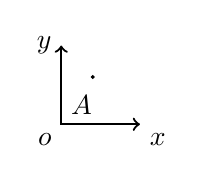
\begin{tikzpicture}
				\draw [thick, <->] (0,1) -- (0,0) -- (1,0);
				\node [below right] 	at (1,0) {$x$};
				\node [left] 			at (0,1) {$y$};
				\node [below left] 	at (0,0) {$o$};
				\draw[fill] 			(.4,.6) circle [radius=.5pt];
				\node[above right] 	(.4,.6) {$A$};
				\end{tikzpicture}
			\end{block}


%				\begin{tikzpicture}
%				\draw [thick, <->] (0,1) -- (0,0) -- (1,0);
%				\node [below right] 	at (1,0) {$x$};
%				\node [left] 			at (0,1) {$y$};
%				\node [below left] 	at (0,0) {$o$};
%				\draw[fill] 			(.4,.6) circle [radius=.5pt];
%				\node[above right] 	(.4,.6) {$A$};
%				\end{tikzpicture}


		\end{column}
		\end{columns}

		\end{frame}





	%	==========================================================
	%		Node
	%	----------------------------------------------------------
		\begin{frame}[t]
		\frametitle{ Node}

				\begin{block}{ Node }
				\begin {itemize}
				\item[] \textbackslash node ( 노드이름 ) at ( 0 , 0 ) \{ 내용 \}
				\item[] \textbackslash node [ shape=형태 ] ( 노드이름 ) [ 위치 ] \{ 내용 \}

				\end {itemize}
				\end{block}


		\end{frame}















	%	==========================================================
	%		예제 : 선의 두께
	%	----------------------------------------------------------
		\begin{frame}[t]
		\frametitle{예제 : 선의 두께}

			\begin{columns}[t]
			\begin{column}{.4\textwidth}
				\begin{block}{선의 두께 종류}
				\begin{description}[12345678901234567890]
				\item	[ultra thin]
				\item 	[very thin]
				\item 	[thin]
				\item 	[semithick]
				\item 	[thick]
				\item 	[very thick]
				\item 	[ultra thick]
				\end{description}
				\end{block}
			\end{column}

	%	----------------------------------------------------------	예제 : 선의 두께 종류
			\begin{column}{.4\textwidth}
				\begin{example}
				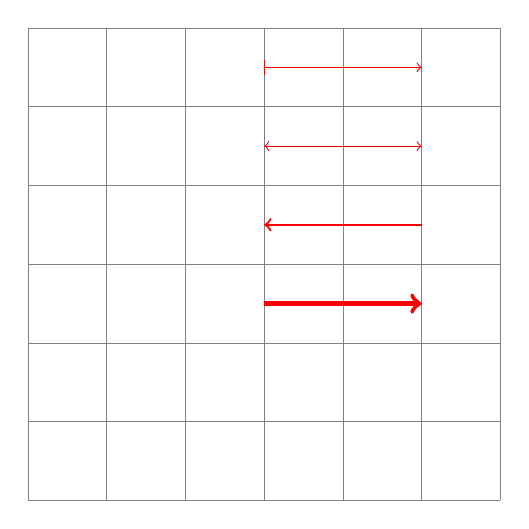
\begin{tikzpicture}[xscale=1.0]
				\draw[help lines, step=1.0, color=gray] (-3 , -3) grid ( 3, 3) ;
				\draw [->] 	[ultra thick	, draw=red] (0,-0.5) -- (2,-0.5);
				\draw [<-]	[thick 		, draw=red] (0,0.5) -- (2,0.5);
				\draw [<->]	[thin		, draw=red] (0,1.5) -- (2,1.5);
				\draw [|->]	[draw=red] (0,2.5) -- (2,2.5);
				\end{tikzpicture}
				\end{example}
			\end{column}
			\end{columns}


	%	----------------------------------------------------------	예제 : 선의 두께 사용자정의
			\begin{block}{선의 두께 : 사용자 정의}
			\end{block}

			\begin{example}
				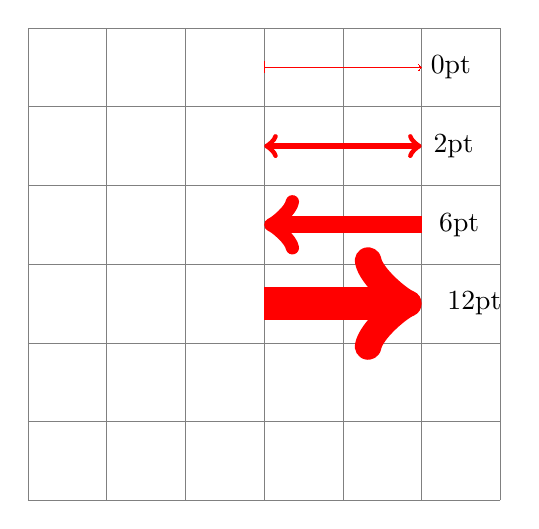
\begin{tikzpicture}[xscale=1.0]
				\draw[help lines, step=1.0, color=gray] (-3 , -3) grid ( 3, 3);
				\draw [->] 	[line width=12pt	, draw=red] (0,-0.5) -- (2,-0.5) 	node [right] {12pt};
				\draw [<-]	[line width=6pt	, draw=red] (0,0.5) -- (2,0.5)		node [right] {6pt};
				\draw [<->]	[line width=2pt	, draw=red] (0,1.5) -- (2,1.5)		node [right] {2pt};
				\draw [|->]	[line width=0pt	, draw=red] (0,2.5) -- (2,2.5)		node [right] {0pt};
				\end{tikzpicture}
			\end{example}

		\end{frame}



	%	==========================================================
	%		예제 : 선의 끝부분 형태
	%	----------------------------------------------------------
		\begin{frame}[t]
		\frametitle{선의 끝부분 형태}

			\begin{example}
				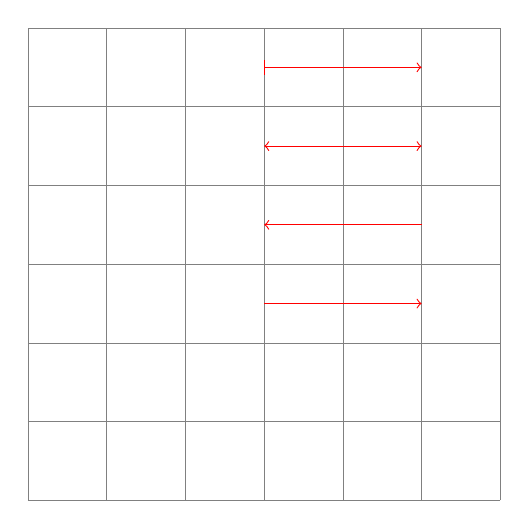
\begin{tikzpicture}[xscale=1.0]
				\draw[help lines, step=1.0, color=gray] (-3 , -3) grid ( 3, 3) ;
				\draw [->] 	[draw=red] (0,-0.5) -- (2,-0.5);
				\draw [<-]	[draw=red] (0,0.5) -- (2,0.5);
				\draw [<->]	[draw=red] (0,1.5) -- (2,1.5);
				\draw [|->]	[draw=red] (0,2.5) -- (2,2.5);
				\end{tikzpicture}
			\end{example}

	%	----------------------------------------------------------
			\begin{block}{선의 끝부분 형태지정을 활용한 좌표축 그림}
			\end{block}

			\begin{example}
				\begin{tikzpicture}[xscale=1.0]
				\draw [<->] 	[draw=red] (0,4) -- (0,0) -- (4,0);
				\end{tikzpicture}
			\end{example}

		\end{frame}


	%	==========================================================
	%		예제 : 선의 종류 : 데쉬와 도트
	%	----------------------------------------------------------
		\begin{frame}[t]
		\frametitle{예제 : 선의 종류 : 데쉬와 도트}

			\begin{example}

				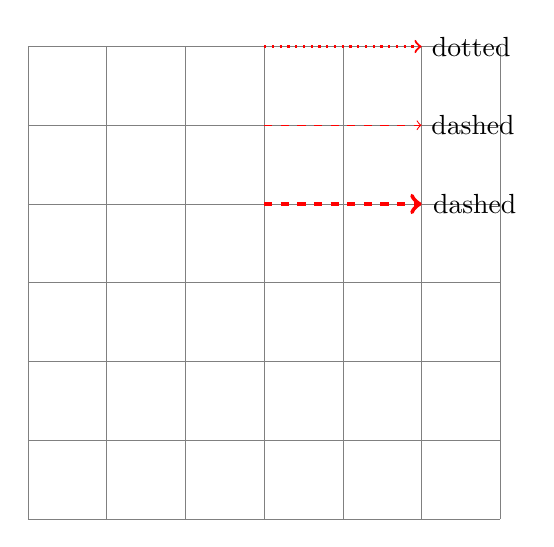
\begin{tikzpicture}[xscale=1.0]
				\draw[help lines, step=1.0, color=gray] (-3 , -3) grid ( 3, 3);
				\draw [->] 	[dashed	,ultra thick	, draw=red] (0,1) -- (2,1) 	node [right] {dashed};
				\draw [->] 	[dashed				, draw=red] (0,2) -- (2,2) 	node [right] {dashed};
				\draw [->] 	[dotted	,thick		, draw=red] (0,3) -- (2,3) 	node [right] {dotted};
				\end{tikzpicture}

			\end{example}

		\end{frame}



	%	==========================================================
	%		예제 : 선의 색깔
	%	----------------------------------------------------------
		\begin{frame}[t]
		\frametitle{선의 색깔}


			\begin{block}{선의 색깔 종류}
			\begin{description}[12345678901234567890]
			\item	[red]		
\begin{tikzpicture}  \draw [->] [ultra thick	, draw=red] (0,1) -- (2,1); \end{tikzpicture}
			\item 	[green]		
\begin{tikzpicture}  \draw [->] [ultra thick	, draw=green] (0,1) -- (2,1); \end{tikzpicture}
			\item 	[blue]		
\begin{tikzpicture}  \draw [->] [ultra thick	, draw=blue] (0,1) -- (2,1); \end{tikzpicture}
			\item 	[cyan]		
\begin{tikzpicture}  \draw [->] [ultra thick	, draw=cyan] (0,1) -- (2,1); \end{tikzpicture}
			\item 	[magenta]		
\begin{tikzpicture}  \draw [->] [ultra thick	, draw=magenta] (0,1) -- (2,1); \end{tikzpicture}
			\item 	[yellow]		
\begin{tikzpicture}  \draw [->] [ultra thick	, draw=yellow] (0,1) -- (2,1); \end{tikzpicture}
			\item 	[black]		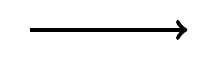
\begin{tikzpicture}  \draw [->] [ultra thick	, draw=black] (0,1) -- (2,1); \end{tikzpicture}
			\item 	[gray]		
\begin{tikzpicture}  \draw [->] [ultra thick	, draw=gray] (0,1) -- (2,1); \end{tikzpicture}
			\item 	[darkgray]	
\begin{tikzpicture}  \draw [->] [ultra thick	, draw=darkgray] (0,1) -- (2,1); \end{tikzpicture}
			\item 	[lightgray]	
\begin{tikzpicture}  \draw [->] [ultra thick	, draw=lightgray] (0,1) -- (2,1); \end{tikzpicture}
			\item 	[brown]		
\begin{tikzpicture}  \draw [->] [ultra thick	, draw=brown] (0,1) -- (2,1); \end{tikzpicture}
			\item 	[lime]		
\begin{tikzpicture}  \draw [->] [ultra thick	, draw=lime] (0,1) -- (2,1); \end{tikzpicture}
			\item 	[olive]		
\begin{tikzpicture}  \draw [->] [ultra thick	, draw=olive] (0,1) -- (2,1); \end{tikzpicture}
			\item 	[orange]		
\begin{tikzpicture}  \draw [->] [ultra thick	, draw=orange] (0,1) -- (2,1); \end{tikzpicture}
			\item 	[pink]		
\begin{tikzpicture}  \draw [->] [ultra thick	, draw=pink] (0,1) -- (2,1); \end{tikzpicture}
			\item 	[purple]		
\begin{tikzpicture}  \draw [->] [ultra thick	, draw=purple] (0,1) -- (2,1); \end{tikzpicture}
			\item 	[teal]		
\begin{tikzpicture}  \draw [->] [ultra thick	, draw=teal] (0,1) -- (2,1); \end{tikzpicture}
			\item 	[violet]		
\begin{tikzpicture}  \draw [->] [ultra thick	, draw=violet] (0,1) -- (2,1); \end{tikzpicture}
			\item 	[white]		\begin{tikzpicture}  \draw [->] [ultra thick	, draw=white] (0,1) -- (2,1); \end{tikzpicture}
			\end{description}
			\end{block}


		\end{frame}


	%	==========================================================
	%		기본 그리기 명령 : 선그리기
	%	----------------------------------------------------------
		\begin{frame}[t]
		\frametitle{기본 그리기 명령 : 선그리기}

			\begin{block}{Draw}
			\begin{itemize}
			\item[] 	\textbackslash draw ( \_ , \_ ) $--$ ( \_ , \_ ) ;
			\item[] 	\textbackslash draw [ verythin, red ] ( \_ , \_ ) \_\_ ( \_ , \_ ) ;
			\end{itemize}
			\end{block}

	%	----------------------------------------------------------
			\begin{example}
				\begin{tikzpicture}
			 	\draw (0,0)--(1,0);
				\end{tikzpicture}
			\end{example}



		%	----------------------------------------------------------
			\begin{block}{Path}
			\begin{itemize}
			\item[] 	\textbackslash path ( a , b )
			\item[] 	\textbackslash path ( $\alpha$ : rim )
					\begin{description}[1234567890]
					\item[$\alpha$] : angle
					\item[rim] : radius
					\end{description}

			\end{itemize}
			\end{block}


		%	----------------------------------------------------------
			\begin{block}{Path [ line ]}
			\end{block}


		%	----------------------------------------------------------
			\begin{example}
			\begin{itemize}
				\item[] \textbackslash tikzstyle\{line\} = [ draw , -latex]
				\item[] \textbackslash begin\{tikzpicture\}
				\item[] \textbackslash path [line] (0,0)--(1,0);
				\item[] \textbackslash end\{tikzpicture\}
			\end{itemize}
			\end{example}

	%	----------------------------------------------------------
			\begin{example}
				\tikzstyle{line} = [ draw , -latex]
				\begin{tikzpicture}
			 	\path [line] (0,0)--(1,0);
				\end{tikzpicture}
			\end{example}

	%	----------------------------------------------------------
			\begin{example}
				\begin{tikzpicture}
			 	\path (0,0);
				\end{tikzpicture}
			\end{example}



		\end{frame}

	%	==========================================================
	%		기본 그리기 명령 : 예제
	%	----------------------------------------------------------
		\begin{frame}[t]
		\frametitle{기본 그리기 명령}

			\begin{example}
			\begin{itemize}
			\item[] 	\textbackslash begin \{ tikzpicture\}
			\item[] 	\% Define the points of a regular pentagon
			\item[] 	\textbackslash path (0,0) coordinate (origin) ;
			\item[] 	\textbackslash path (0 : 1cm) coordinate (P0 ) ;
			\item[] 	\textbackslash path (1*72 : 1cm) coordinate (P1 ) ;
			\item[] 	\textbackslash path (2*72 : 1cm) coordinate (P2 ) ;
			\item[] 	\textbackslash path (3*72 : 1cm) coordinate (P3 ) ;
			\item[] 	\textbackslash path (4*72 : 1cm) coordinate (P4 ) ;
			\item[] 	\% Define the points of a regular pentagon
			\item[] 	\textbackslash draw (p0) $--$ (p1) $--$ (p2) $--$ (p3) $--$ (p4) $--$ cycle;
			\item[] 	\% Add spokes
			\item[] 	\textbackslash draw (origin) $--$ (p0) (origin) $--$ (p1) 
								(origin) $--$ (p2) (origin) $--$ (p3) (origin) $--$ (p4);
			\item[] 	\textbackslash end \{tikzpicture \}
			\end{itemize}
			\end{example}

			\begin{example}
				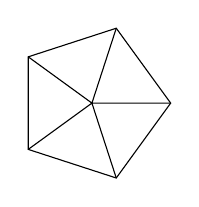
\begin{tikzpicture}
			 	\path (0,0) coordinate (origin) ;
				\path (0 : 1cm) 	coordinate (p0) ;
				\path (1*72 : 1cm) coordinate (p1) ;
				\path (2*72 : 1cm) coordinate (p2) ;
				\path (3*72 : 1cm) coordinate (p3) ;
				\path (4*72 : 1cm) coordinate (p4) ;
				\draw (p0)--(p1)--(p2)--(p3)--(p4)--cycle;
				\draw (origin)--(p0) (origin)--(p1) (origin)--(p2) (origin)--(p3) (origin)--(p4);
				\end{tikzpicture}
			\end{example}

		\end{frame}





	%	==========================================================
	%		기본 그리기 명령 : node
	%	----------------------------------------------------------
		\begin{frame}[t]
		\frametitle{기본 그리기 명령 : node}

			\begin{block}{node}
			\end{block}

		%	-----------------------------------------------------
			\begin{block}{node block}
			\begin{itemize}
			\item[] 	\textbackslash tikzstyle \{block\} = [ rectangle, draw, text width=6em, text height=1em]
			\item[] 	\textbackslash tikzstyle\{line\} = [ draw , -latex]
			\item[] 	\textbackslash begin\{tikzpicture\}[node distance = 8em and 2em, auto]
			\item[] 	
			\item[] 	\textbackslash node [block] (b0) 				{ 0000 }
			\item[] 	\textbackslash node [block, left of=b0 ] (b1) 	{ 1111 }
			\item[] 	\textbackslash node [block, right of=b0 ] (b2) 	{ 1111 }
			\item[] 	\textbackslash node [block, below of=b0 ] (b3) 	{ 1111 }
			\item[] 	\textbackslash node [block, below of=b3 ] (b4) 	{ 1111 }
			\item[] 	\textbackslash path [line] (b0) $--$ (b1)
			\item[] 	\textbackslash path [line] (b0) $--$ (b2)
			\item[] 	\textbackslash path [line] (b0) $--$ (b3)
			\item[] 	\textbackslash path [line] (b3) $--$ (b4)
			\item[] 	\textbackslash end\{tikzpicture\}

			\end{itemize}
			\end{block}

			\begin{itemize}
			\item block스타일 정의에서 넓이
			\item block스타일 정의에서 높이
			\item line의 -retex의 의미
			\item block의 배치
					\begin{itemize}
					\item left
					\item right
					\item below
					\item above
					\end{itemize}
			\end{itemize}
			distance의 8 과 2의 의미


		%	-----------------------------------------------------
			\begin{block}{node}
	
				\tikzstyle{block} = [ rectangle, draw, text width=6em, text height=1em]
				\tikzstyle{line} = [ draw , -latex]
	
				\begin{tikzpicture}[node distance = 8em and 2em, auto]
				\node [block] (b0) 				{ 0000 };
				\node [block, left of=b0 ] (b1) 	{ 1111 };
				\node [block, right of=b0 ] (b2) 	{ 2222 };
				\node [block, below of=b0 ] (b3) 	{ 3333 };
				\node [block, below of=b3 ] (b4) 	{ 4444 };
	
				\path [line] (b0)--(b1);
				\path [line] (b0)--(b2);
				\path [line] (b0)--(b3);
				\path [line] (b3)--(b4);
	
				\end{tikzpicture}
	
			\end{block}

		\end{frame}



			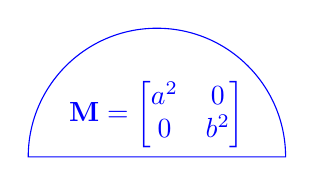
\begin{tikzpicture}
			\node [semicircle, draw, blue] {$\mathbf{M} = \begin{bmatrix}a^2 & 0 \\0 & b^2 \\\end{bmatrix}$};
			\end{tikzpicture}



			\usetikzlibrary{shadows}


			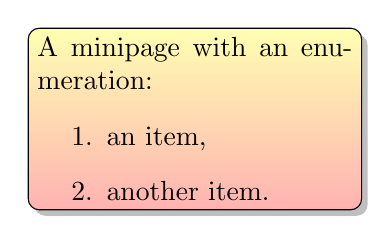
\begin{tikzpicture}
			\node [rectangle, rounded corners,draw, drop shadow, shade,top color=yellow!30,bottom color=red!30] {
					\begin{minipage}{4cm}%
					A minipage with an enumeration:
					\begin{enumerate}
					\item an item,
					\item another item.
					\end{enumerate}
					\end{minipage}
					};
			\end{tikzpicture}










	%	----------------------------------------------------------
	%		positing 라이버러리 사용
	%	----------------------------------------------------------

		\begin{frame}[t]
		\frametitle{positing 라이버러리 사용}

			\begin{block}{node distance}

			\begin{itemize}
			\item[] 	\textbackslash node [block, below of=b0 ] (b3) \{ 3333 \};
			\item[] 	\textbackslash node [block, below=2em of b0 ] (b3) \{ 3333 \};
			\end{itemize}

			\end{block}

			\begin{block}{xshift, yshift}

			\begin{itemize}
			\item[] 	xshift = -2em
			\item[] 	yshift = -2em
			\end{itemize}

			\end{block}


		%	-----------------------------------------------------
			\begin{block}{node distance}

			\begin{itemize}
			\item[] 	\textbackslash begin\{tikzpicture\}[node distance = 8em and 2em, auto]
			\end{itemize}

			\end{block}
	

		\end{frame}



	%	==========================================================
	%		Placing Nodes
	%	----------------------------------------------------------

		\begin{frame}[t]
		\frametitle{Placing Nodes}

			\begin{block}{Placing Nodes Using at syntax}
			\begin{itemize}
			\item[] 	\textbackslash node at ( $-$ , $-$ )
			\end{itemize}
			\end{block}

			\begin{block}{Placing Nodes Using Relative Placement}
			\begin{itemize}
			\item[] 	\textbackslash node [below of=$--$ ] (b3) \{ 3333 \};
			\item[] 	\textbackslash node [above of=$--$ ] (b3) \{ 3333 \};
			\item[] 	\textbackslash node [left of=$--$ ] (b3) \{ 3333 \};
			\item[] 	\textbackslash node [right of=$--$ ] (b3) \{ 3333 \};
 			\end{itemize}
			\end{block}

			\begin{block}{Placing Nodes Using Anchors}
			\begin{itemize}
			\item[] 	\textbackslash node [anchor=north west] (b3) \{ 3333 \};
			\item[] 	\textbackslash node [anchor=north ] (b3) \{ 3333 \};
			\item[] 	\textbackslash node [anchor=north east] (b3) \{ 3333 \};
			\item[] 	\textbackslash node [anchor=west] (b3) \{ 3333 \};
			\item[] 	\textbackslash node [anchor=east] (b3) \{ 3333 \};
			\item[] 	\textbackslash node [base] (b3) \{ 3333 \};
 			\end{itemize}
			\end{block}

	
		\end{frame}


	%	----------------------------------------------------------


			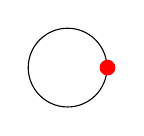
\begin{tikzpicture}
			\node [circle, draw, minimum size=1cm] (c) {};
			\path [fill=red] (c.east) circle (1mm);
			\end{tikzpicture}





	%	==========================================================
	%		영역 채우기
	%	----------------------------------------------------------













	%	==========================================================
	%		Tikz Style
	%	----------------------------------------------------------
		\begin{frame}[t]
		\frametitle{Tikz Style}

			\begin{block}{Tikz Style}
			\begin{itemize}
			\item[] 	\textbackslash tikzstyle \{block\} = [ rectangle, draw, text width=6em, text height=1em]
			\item[] 	\textbackslash tikzstyle\{line\} = [ draw , -latex]
			\end{itemize}
			\end{block}


			\begin{block}{width, height}
			\begin{itemize}
			\item[] 	text width = 6em
			\item[] 	text height = 6em
			\item[] 	minimum width = 6em
			\item[] 	minimum height = 6em
			\end{itemize}
			\end{block}



	
		%	----------------------------------------------------------

			\begin{block}{Tikz Style}
			\begin{itemize}
			\item[] 	round corners
			\item[] 	text centered
			\item[] 	draw=black
			\item[] 	fill=red!30
			\end{itemize}
			\end{block}


	


	%	----------------------------------------------------------
	
			\begin{block}{trapezium}
			\begin{itemize}
			\item[] 	trapezium left angle=70
			\item[] 	trapezium right angle=110
			\end{itemize}
			\end{block}


		\end{frame}



	%	==========================================================
	%		Shape Library
	%	----------------------------------------------------------

		\begin{frame}[plain]

			\centering
			\scalebox{4}{Shape Library}
	
		\end{frame}



	%	----------------------------------------------------------
	%		Shape Library
	%	----------------------------------------------------------
		\begin{frame}[t]
		\frametitle{Shape Library: Predefined Shapes}

			\begin{block}{shape}
			\begin{itemize}
			\item[] 	circle
			\item[] 	diamond
			\item[] 	ellipse
			\item[] 	trapezium
			\item[] 	semicircle
			\item[] 	regular polygon
			\item[] 	star
			\item[] 	isosceles triangle
			\item[] 	kite
			\item[] 	dart
			\item[] 	circular sector
			\item[] 	cylinder
			\item[] 	rectangle
			\item[] 	coordinate
			\end{itemize}
			\end{block}

				
\begin{tikzpicture}
				\node [shape=circle, draw, minimum size=1cm] (c) {};
				\end{tikzpicture}
				
\begin{tikzpicture}
				\node [diamond, draw, minimum size=1cm] (c) {};
				\end{tikzpicture}
				
\begin{tikzpicture}
				\node [ellipse, draw, minimum size=1cm] (c) {};
				\end{tikzpicture}
				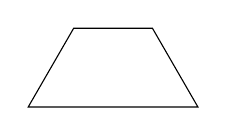
\begin{tikzpicture}
				\node [trapezium, draw, minimum size=1cm] (c) {};
				% trapezium left angle=120
				% trapezium right angle=120
				\end{tikzpicture}
				% --------------------
				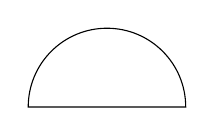
\begin{tikzpicture}
				\node [shape=semicircle, draw, minimum size=1cm] (c) {};
				\end{tikzpicture}
				% --------------------
				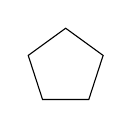
\begin{tikzpicture}
				\node [shape=regular polygon, draw, minimum size=1cm] (c) {};
				\end{tikzpicture}
				% --------------------
				
\begin{tikzpicture}
				\node [shape=star, draw, minimum size=1cm] (c) {};
				\end{tikzpicture}
				% star points=<integer>
				% star point height=<distance>
				% star point ration=<number>
				% --------------------
				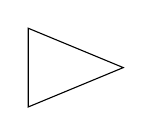
\begin{tikzpicture}
				\node [shape=isosceles triangle, draw, minimum size=1cm] (c) {};
				\end{tikzpicture}
				% --------------------
				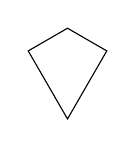
\begin{tikzpicture}
				\node [shape=kite	, draw, minimum size=1cm] (c) {};
				\end{tikzpicture}
				% --------------------
				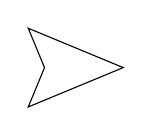
\begin{tikzpicture}
				\node [shape=dart	, draw, minimum size=1cm] (c) {};
				\end{tikzpicture}
				% --------------------
				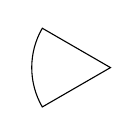
\begin{tikzpicture}
				\node [shape=circular sector, draw, minimum size=1cm] (c) {};
				\end{tikzpicture}
				% --------------------
				
\begin{tikzpicture}
				\node [shape=cylinder, draw, minimum size=1cm] (c) {};
				\end{tikzpicture}
				% --------------------
				
\begin{tikzpicture}
				\node [rectangle	, draw, minimum size=1cm] (c) {};
				\end{tikzpicture}
				% --------------------
				\begin{tikzpicture}
				\node [shape=coordinate, draw, minimum size=1cm] (c) {};
				\end{tikzpicture}

	%	----------------------------------------------------------
			\begin{columns}[t]
			\begin{column}{.6\textwidth}
			\begin{block} {원 그리기 예제}
			\begin{itemize}
				\item[] \textbackslash begin \{tikzpicture\}
				\item[] \textbackslash draw (0,0) circle (0.5);
				\item[] \textbackslash end\{tikzpicture\}
			\end{itemize}
			\end{block}
			\end{column}


			\begin{column}{.4\textwidth}
			\begin{example}
				
\begin{tikzpicture}[xscale=1.0]
				\draw (0,0) circle (0.5);
				\end{tikzpicture}
			\end{example}
			\end{column}
			\end{columns}


	%	----------------------------------------------------------
			\begin{columns}[t]
			\begin{column}{.6\textwidth}
			\begin{block} {원 그리기 예제}
			\begin{itemize}
				\item[] \textbackslash begin \{tikzpicture\}
				\item[] \textbackslash path node [shape=circle, draw, color=red] \{hello\};
				\item[] \textbackslash end\{tikzpicture\}
			\end{itemize}
			\end{block}
			\end{column}


			\begin{column}{.4\textwidth}
			\begin{example}
				\begin{tikzpicture}[xscale=1.0]
				\path node [shape=circle, draw, color=red] {hello};
				\end{tikzpicture}
			\end{example}
			\end{column}
			\end{columns}


	%	----------------------------------------------------------
			\begin{columns}[t]
			\begin{column}{.6\textwidth}
			\begin{block} {원 그리기 예제}
			\begin{itemize}
				\item[] \textbackslash begin \{tikzpicture\}
				\item[] \textbackslash draw [blue] (0,0) rectangle (2,4);
				\item[] \textbackslash draw[blue,thick] (0,0) circle [radius=1cm] ;
				\item[] \textbackslash draw[blue,thick] (0,0) circle [radius=1.414cm] ;
				\item[] \textbackslash draw[blue,thick] (0,0) circle [radius=2cm] ;
				\item[] \textbackslash end\{tikzpicture\}
			\end{itemize}
			\end{block}
			\end{column}


			\begin{column}{.4\textwidth}
			\begin{example}
				\begin{tikzpicture}[xscale=1.0]
				\draw[blue,thick] (0,0) circle [radius=1cm] ;
				\draw[blue,thick] (0,0) circle [radius=1.414cm] ;
				\draw[blue,thick] (0,0) circle [radius=2cm] ;
				\end{tikzpicture}
			\end{example}
			\end{column}
			\end{columns}

		\end{frame}


	%	==========================================================
	%		Symbol Shape Library
	%	----------------------------------------------------------
		\begin{frame}[t]
		\frametitle{Shape Library: Symbol Shapes}

			\begin{block}{shape}
			\begin{itemize}
			\item[] 	forbidden sign
			\item[] 	magnifying glass
			\item[] 	cloud
			\item[] 	starburst
			\item[] 	signal
			\item[] 	tape
			\end{itemize}
			\end{block}

		\end{frame}






	%	==========================================================
	%		Arrow Shape Library
	%	----------------------------------------------------------
		\begin{frame}[t]
		\frametitle{Shape Library: Arrow Shapes}

			\begin{block}{Arrow shape}
			\end{block}

		\end{frame}






	%	==========================================================
	%		Shapes with Multple Text parts
	%	----------------------------------------------------------
		\begin{frame}[t]
		\frametitle{Shape Library: Shapes with Multple Text parts}

			\begin{block}{Shapes with Multple Text parts}
			\end{block}

		\end{frame}




	%	==========================================================
	%		Callout Shapes
	%	----------------------------------------------------------
		\begin{frame}[t]
		\frametitle{Shape Library: Callout Shapes}

			\begin{block}{Callout Shapes}
			\end{block}

		\end{frame}

	%	==========================================================
	%		Text
	%	----------------------------------------------------------
		\begin{frame}[plain]

			\centering
			\scalebox{4}{Text}
	
		\end{frame}


	%	----------------------------------------------------------
		\begin{frame}
		\frametitle{Text}

		\begin{block}{Text 배치}
			\begin{tikzpicture}
			\draw [thick, <->] (0,2) -- (0,0) -- (2,0);
			\node at (1,1) { yes };
			\end{tikzpicture}

		\end{block}


		\begin{block}{아래위 좌우에 배치}
			\begin{tikzpicture}
			\draw [thick, <->] (0,2) -- (0,0) -- (2,0);
			\draw[fill] (1,1) circle [radius=0.025];
			\node [below]	at (1,1) {below};
			\node [above]	at (1,1) {above};
			\node [left]	at (1,1) {left};
			\node [right]	at (1,1) {right};
			\end{tikzpicture}
		\end{block}

		\begin{block}{혼합해서 배치}
			\begin{tikzpicture}[scale=2]
			\draw 	[thick, <->] (0,1) -- (0,0) -- (1,0);
			\draw	[fill] (1,1) circle [radius=0.025];
			\node	[below right, red] 	at (1,1) {below right};
			\node	[above left, green] 	at (1,1) {above left};
			\node	[below left, purple] 	at (1,1) {below left};
			\node	[above right, magenta] at (1,1) {above right};
			\end{tikzpicture}
		\end{block}


		\begin{tikzpicture}[xscale=3, yscale=1.5]
			\draw [thick, <->] (0,1) -- (0,0) -- (1,0);
			\node [below right] 	at (1,0) {$x$};
			\node [left] 			at (0,1) {$y$};
			\draw[fill] 			(.4,.6) circle [radius=.5pt];
			\node[above right] 	(.4,.6) {$A$};
		\end{tikzpicture}



		\end{frame}









\tikzstyle{shaded}=[fill=red!10!blue!20!gray!50!white]
\tikzstyle{shaded line}=[double=red!10!blue!20!gray!50!white, double distance=2mm, draw=black]
\tikzstyle{unshaded}=[fill=white]
\tikzstyle{unshaded line}=[double=white, double distance=2mm, draw=black]
\tikzstyle{Tbox}=[circle, draw, thick, fill=white, opaque,]
\tikzstyle{empty box}=[circle, draw, thick, fill=white, opaque, inner sep=2mm]
\tikzstyle{background rectangle}= [fill=red!10!blue!20!gray!40!white,rounded corners=2mm] 
\tikzstyle{on}=[very thick, red!50!blue!50!black]
\tikzstyle{off}=[gray]

%These are for resizing a family of drawings at the same time
\tikzstyle{traces}=[scale=.2, inner sep=1mm,baseline]
\tikzstyle{quadratic}=[scale=.23, inner sep=.5mm, baseline]
\tikzstyle{annular}=[scale=.6, inner sep=1mm, baseline]
\tikzstyle{make triple edge size}= [scale=.4, inner sep=1mm,baseline] 
\tikzstyle{icosahedron network}=[scale=.35, inner sep=1mm, baseline]
\tikzstyle{ATLsix}=[scale=.25, baseline]
\tikzstyle{TL12}=[scale=.15,baseline=-0.5ex]

% I added the "=-0.5ex" -SB
\tikzstyle{TLEG}=[scale=.5,baseline]
\tikzstyle{PAdefn}=[scale=.7,baseline]
\tikzstyle{STrain}=[baseline=0,scale=2]























	%	========================================================== flowchart
	%		flowchart
	%	----------------------------------------------------------

		\begin{frame}[plain]

			\centering
			\scalebox{4}{flowchart}
	
		\end{frame}



	%	----------------------------------------------------------
		\begin{frame}[t]{flowchart}


			
			\begin{block}{flowchart 사용준비 }
			\begin{itemize}
			\item[] \textbackslash usepackage \{flowchart\}
			\item[] \textbackslash usetikzlibrary \{arrows\}
			\end{itemize}
			\end{block}

			\begin{columns}[t]

			\begin{column}{.18\textwidth}
			\begin{block} { Process}
					\centering
					\vskip 2mm
					\begin{tikzpicture}
					\node (node01) at (0,0) [draw, terminal, minimum width=2cm, minimum height=1cm] {terminal};
					\end{tikzpicture}
					\vskip 2mm
			\end{block}
			\end{column}


			\begin{column}{.18\textwidth}
			\begin{block} { Decision}
					\centering
					\vskip 2mm
					\begin{tikzpicture}
					\node (node01) at (0,0) [draw, decision, minimum width=2cm, minimum height=1cm] {decision};
					\end{tikzpicture}
					\vskip 2mm
			\end{block}
			\end{column}


			\begin{column}{.18\textwidth}
			\begin{block} {Predefined Process}
					\centering
					\vskip 2mm
					\begin{tikzpicture}
					\node (node01) at (0,0) [draw, predproc, minimum width=2cm, minimum height=1cm] {predproc};
					\end{tikzpicture}
					\vskip 2mm
			\end{block}
			\end{column}


			\begin{column}{.18\textwidth}
			\begin{block} { Storage}
					\centering
					\vskip 2mm
					\begin{tikzpicture}
					\node (node01) at (0,0) [draw, storage, minimum width=2cm, minimum height=1cm] {storage};
					\end{tikzpicture}
					\vskip 2mm
			\end{block}
			\end{column}


			\begin{column}{.18\textwidth}
			\begin{block} { Terminal}
					\centering
					\vskip 2mm
					\begin{tikzpicture}
					\node (node01) at (0,0) [draw, terminal, minimum width=2cm, minimum height=1cm] {teminal};
					\end{tikzpicture}
					\vskip 2mm
			\end{block}
			\end{column}

			\end{columns}



				\begin{tikzpicture}
				\def\smbwd{2cm}
				\node (terminal1)		at (0,0) 		[draw, terminal,minimum width=\smbwd,minimum height=0.5cm] {START};
				\node (predproc1) 		at (0,-1.5) 	[draw, predproc, align=left,minimum width=\smbwd,minimum height=1cm] {GET\\ DATA};
				\node (decide1) 		at (0,-3.5) 	[draw, decision, minimum width=\smbwd, minimum height=1cm] {C$<$3};
				\node (storage1) 		at (0,-5.5) 	[draw, storage, minimum width=\smbwd, minimum height=1cm] {STORE};
				\node (process1) 		at (3,-5.5) 	[draw, process, minimum width=\smbwd, minimum height=1cm] {PROCESS};
				\coordinate (point1) 	at (0,-6.75);
				\node (terminal2) 		at (0,-7.75) [draw, terminal, minimum width=\smbwd, minimum height=0.5cm] {END};
				\draw[->] (terminal1) -- (predproc1);
				\draw[->] (predproc1) -- (decide1);
				\draw[->] (decide1) -| node[above]{YES} (process1);
				\draw[->] (decide1) -- (storage1);
				\draw[->] (process1) |- (point1);
				\draw[->] (storage1) -- (point1) -- (terminal2);
				\end{tikzpicture}







		\end{frame}





	%	==========================================================
	%		structural analysis
	%	----------------------------------------------------------

		\begin{frame}[plain]

			\centering
			\scalebox{4}{구조계산 그림}
	
		\end{frame}


	%	----------------------------------------------------------
		\begin{frame}[t,shrink=0]{특수문자 : 구조 계산 그림용 package marvosym}


			\begin{block}{특수문자 : 구조 계산 그림용 package marvosym}
			\begin{itemize}
			\item[] \textbackslash usepackage \{marvosys\}
			\end{itemize}
			\end{block}

			\begin{columns}[t]
			\begin{column}{.4\textwidth}
			\begin{block} { 모델링 }

			\begin{enumerate}
			\item[\Beam			]	\textbackslash Beam	
			\item[\Force			]	\textbackslash Force	
			\item[\Lineload		]	\textbackslash Lineload	
			\item[\Lefttorque		]	\textbackslash Lefttorque	
			\item[\Righttorque		]	\textbackslash Righttorque	
			\item[\Fixedbearing	]	\textbackslash Fixedbearing	
			\item[\Bearing		]	\textbackslash Bearing
			\item[\Loosebearing	]	\textbackslash Loosebearing	

			\item[\Rectpipe		]	\textbackslash Rectpipe
			\item[\Squarepipe		]	\textbackslash Squarepipe	
			\item[\Circpipe		]	\textbackslash Circpipe	
			\end{enumerate}

			\end{block}
			\end{column}

			\begin{column}{.4\textwidth}
			\begin{block} { 단면 }
			\begin{enumerate}
			\item[\Circsteel		]	\textbackslash Circsteel	
			\item[\Octosteel		]	\textbackslash Octosteel	
			\item[\Hexasteel		]	\textbackslash Hexasteel
			\item[\Squaresteel•		]	\textbackslash Squaresteel•	
			\item[\Rectsteel		]	\textbackslash Rectsteel	

			\item[\Tsteel			]	\textbackslash Tsteel	
			\item[\RoundedTsteel	]	\textbackslash RoundedTsteel	
			\item[\TTsteel		]	\textbackslash TTsteel	
			\item[\RoundedTTsteel	]	\textbackslash RoundedTTsteel
			\item[\Flatsteel		]	\textbackslash Flatsteel	
			\item[\Lsteel			]	\textbackslash Lsteel	
			\item[\RoundedLsteel	]	\textbackslash RoundedLsteel	
			\end{enumerate}
			\end{block}
			\end{column}
			\end{columns}

		\end{frame}




	%	==========================================================
	%		structural analysis
	%	----------------------------------------------------------



		\begin{frame}[t]{structuralan alysis : 사용준비 }


			\begin{block}{structural analysis 사용준비}
			\begin{itemize}
			\item[] \textbackslash usepackage\{structuralanalysis\}
			\item[] \textbackslash usepackage\{3dstructuralanalysis\}
			\end{itemize}
			\end{block}



			\begin{example}
					\centering
					\vskip 2mm
					\resizebox{0.4\textwidth}{!}{
					\begin{tikzpicture}
		
					\point{a}{0}{0};
					\point{b}{10}{0};
		
					\notation{1}{a}{A};
					\notation{1}{b}{B};
		
					\beam{2}{a}{b}[0][1];
					\support{1}{a}[0];
					\support{1}{b}[0];
					\dimensioning{1}{a}{b}{-1.5}[10m]
					\end{tikzpicture}
					}
					\vskip 2mm	
			\end{example}

			\begin{itemize}
			\item[] \textbackslash begin\{tikzpicture\}
			\item[] \textbackslash point\{a\}\{0\}\{0\}; \textbackslash point\{\b\}\{10\}\{0\};
			\item[] \textbackslash notation\{1\}\{a\}\{A\};	 \textbackslash notation\{1\}\{b\}\{B\};
			\item[] \textbackslash beam\{2\}\{a\}\{b\}[0][1];
			\item[] \textbackslash support\{1\}\{a\}[0]; \textbackslash support\{1\}\{b\}[0];
			\item[] \textbackslash dimensioning\{1\}\{a\}\{b\}\{-1.5\}[10m]
			\item[] \textbackslash end\{tikzpicture\}
			\end{itemize}


		\end{frame}

	%	==========================================================
	%		structural analysis
	%	----------------------------------------------------------



		\begin{frame}[t]{structural analysis : 명령어}
 
			\begin{block}{structural analysis 사용준비}
			\begin{itemize}
			\item[] \textbackslash scaling 
			\item[] \textbackslash point 
			\item[] \textbackslash beam 
			\item[] \textbackslash support
			\item[] \textbackslash hinge
			\item[] \textbackslash load 
			\item[] \textbackslash lineload
			\item[] \textbackslash temperature
			\item[] \textbackslash internalforces
			\item[] \textbackslash dimensioning
			\item[] \textbackslash influenceline
			\item[] \textbackslash notation
			\item[] \textbackslash addon
			\end{itemize}
			\end{block}


		\end{frame}



	%	----------------------------------------------------------
	%	scaling
	%	----------------------------------------------------------

		\begin{frame}[t]{scaling}
 
			\begin{block}{scaling}
			\begin{itemize}
			\item[] \textbackslash scaling \{scaling\_value\};
			\end{itemize}
			\end{block}




		\end{frame}


	%	----------------------------------------------------------
	%	point
	%	----------------------------------------------------------

		\begin{frame}[t]{point}
 
			\begin{block}{point}
			\begin{itemize}
			\item[] \textbackslash point\{name\}\{x-coordiante\}\{y-coordiante\};
			\end{itemize}
			\end{block}


		\end{frame}


	%	----------------------------------------------------------
	%	beam
	%	----------------------------------------------------------

		\begin{frame}[t]{beam}
 
			\begin{block}{beam}
			\begin{itemize}
			\item[]	\textbackslash beam\{type\}\{initial point\}\{end point\}
					[rounded initial point][rounded end point];
			\end{itemize}
			\end{block}


			\begin{block}{beam}
			\begin{description}[12345678901234567890]
%			\item[Biegebalken mit Kennfaser]
			\item[beam + 보강재]
					\textbackslash beam\{1\} \par
					\{initial point\} \par
					\{end point[rounded initial point][rounded end point]\};
%			\item[Fachwerkstab]
			\item[truss]
					\textbackslash beam\{2\}\{initial point\}\{end point\} \par
					[rounded initial point][rounded end point];
%			\item[Unsichtbarer Stab]
			\item[보이지 않는 부재]
					\textbackslash beam\{3\}\{initial point\}\{end point\};
%			\item[Biegebalken ohne Kennfaser]
			\item[Beam]
					\textbackslash beam\{4\}\{initial point\}\{end point\} \par
					[rounded initial point][rounded end point];

			\end{description}
			\end{block}

			\begin{columns}
			\begin{column}{0.25\textwidth}
				\begin{block}{typ 1}
					\centering
					\begin{tikzpicture}
					\scaling{0.5};
					\point{a}{0}{0};
					\point{b}{5}{0};
					\notation{1}{a}{A};
					\notation{1}{b}{B}{right=2};
					\beam{1}{a}{b}[0][1];
					\end{tikzpicture}
				\end{block}
			\end{column}

			\begin{column}{0.25\textwidth}
				\begin{block}{typ 2}
					\centering
					\begin{tikzpicture}
					\scaling{0.5};
					\point{a}{0}{0};
					\point{b}{5}{0};
					\notation{1}{a}{A};
					\notation{1}{b}{B}{right=2};
					\beam{2}{a}{b}[0][1];
					\end{tikzpicture}
				\end{block}
			\end{column}

			\begin{column}{0.25\textwidth}
				\begin{block}{typ 3}
					\centering
					\begin{tikzpicture}
					\scaling{0.5};
					\point{a}{0}{0};
					\point{b}{5}{0};
					\notation{1}{a}{A};
					\notation{1}{b}{B}{right=2};
					\beam{3}{a}{b}[0][1];
					\end{tikzpicture}
				\end{block}
			\end{column}

			\begin{column}{0.25\textwidth}
				\begin{block}{typ 4}
					\centering
					\begin{tikzpicture}
					\scaling{0.5};
					\point{a}{0}{0};
					\point{b}{5}{0};
					\notation{1}{a}{A};
					\notation{1}{b}{B}{right=2};
					\beam{4}{a}{b}[0][1];
					\end{tikzpicture}
				\end{block}
			\end{column}

			\end{columns}




		\end{frame}

	%	----------------------------------------------------------
	%	support
	%	----------------------------------------------------------

		\begin{frame}[t]{support}
 
			\begin{block}{support}
			\begin{itemize}
			\item[] \textbackslash support\{type\}\{insertion point\}[rotation];
			\end{itemize}
			\end{block}


			\begin{block}{support}
			\begin{description}[12345678901234567890]
			\item[Festlager] : 	\textbackslash support\{1\}\{insertion point\}[rotation];
			\item[Loslager]  : 	\textbackslash support\{2\}\{insertion point\}[rotation];
			\item[Einspannung] : \textbackslash support\{3\}\{insertion point\}[rotation];
			\item[Lose Einspannung] : 
								\textbackslash support\{4\}\{insertion point\}[rotation];
			\item[Wegfeder] : 	\textbackslash support\{5\}\{insertion point\}[rotation];
			\item[Drehfeder] : 	\textbackslash support\{6\}\{insertion point\}[rotation];
			\end{description}
			\end{block}

			\begin{columns}[t]
			\begin{column}{0.15\textwidth}
				\begin{block}{typ 1}
					\begin{tikzpicture}
					\scaling{0.2};
					\point{a}{0}{0};
					\point{b}{5}{0};
					\notation{1}{a}{A};
					\notation{1}{b}{B}{right=2};
					\beam{2}{a}{b}[0][1];
					\support{1}{a};
					\end{tikzpicture}
				\end{block}
			\end{column}

			\begin{column}{0.15\textwidth}
				\begin{block}{typ 2}
					\begin{tikzpicture}
					\scaling{0.2};
					\point{a}{0}{0};
					\point{b}{5}{0};
					\notation{1}{a}{A};
					\notation{1}{b}{B}{right=2};
					\beam{2}{a}{b}[0][1];
					\support{2}{a};
					\end{tikzpicture}
				\end{block}
			\end{column}

			\begin{column}{0.15\textwidth}
				\begin{block}{typ 3}
					\begin{tikzpicture}
					\scaling{0.2};
					\point{a}{0}{0};
					\point{b}{0}{5};
					\notation{1}{a}{A};
					\notation{1}{b}{B}{right=2};
					\beam{2}{a}{b}[0][1];
					\support{3}{a};
					\end{tikzpicture}
				\end{block}
			\end{column}


			\begin{column}{0.15\textwidth}
				\begin{block}{typ 4}
					\begin{tikzpicture}
					\scaling{0.2};
					\point{a}{0}{0};
					\point{b}{0}{5};
					\notation{1}{a}{A};
					\notation{1}{b}{B}{right=2};
					\beam{2}{a}{b}[0][1];
					\support{4}{a};
					\end{tikzpicture}
				\end{block}
			\end{column}

			\begin{column}{0.15\textwidth}
				\begin{block}{typ 5}
					\begin{tikzpicture}
					\scaling{0.2};
					\point{a}{0}{0};
					\point{b}{5}{0};
					\notation{1}{a}{A};
					\notation{1}{b}{B}{right=2};
					\beam{2}{a}{b}[0][1];
					\support{5}{a};
					\end{tikzpicture}
				\end{block}
			\end{column}

			\begin{column}{0.15\textwidth}
				\begin{block}{typ 6}
					\begin{tikzpicture}
					\scaling{0.2};
					\point{a}{0}{0};
					\point{b}{5}{0};
					\notation{1}{a}{A};
					\notation{1}{b}{B}{right=2};
					\beam{2}{a}{b}[0][1];
					\support{6}{a};
					\end{tikzpicture}
				\end{block}
			\end{column}

			\end{columns}

		\end{frame}

	%	----------------------------------------------------------
	%	hinge
	%	----------------------------------------------------------

		\begin{frame}[t]{hinge}
 
			\begin{block}{hinge}
			\begin{itemize}
			\item[] \textbackslash hinge\{type\}\{insertion point\}[optional][optional][optional];
			\end{itemize}
			\end{block}

			\begin{block}{hinge}
			\begin{description}[123456789012345678901234567890]
			\item[Vollgelenk : 완전힌지] 			\textbackslash hinge\{1\}\{insertion point\};
			\item[Halbgelenk : 반힌지] 				\textbackslash hinge\{2\}\{insertion point\}[initial point][end point]\par[orientation];
			\item[Querkraftgelenk : 전단력공동] 		\textbackslash hinge\{3\}\{insertion point\}[rotation];
			\item[Normalkraftgelenk] 				\textbackslash hinge\{4\}\{insertion point\}[rotation];
			\item[Aussteifung der Ecken : 코너 보강] 	\textbackslash hinge\{5\}\{insertion point\}[initial point][end point];
			\end{description}
			\end{block}


			\begin{columns}[t]

			\begin{column}{0.20\textwidth}
			\begin{block}{typ 1}
				\begin{tikzpicture}[xscale=0.5, yscale=0.5]
				\scaling{0.2};
				\point{a}{0}{0};
				\point{b}{3}{0};
				\point{c}{6}{0};
				\beam{2}{a}{b}[0][0];
				\beam{2}{b}{c}[0][0];

				\hinge{1}{b};

				\support{1}{a};
				\support{1}{c};
				\end{tikzpicture}
			\end{block}
			\end{column}

			\begin{column}{0.20\textwidth}
			\begin{block}{typ 2}
				\begin{tikzpicture}[xscale=0.5, yscale=0.5]
				\scaling{0.2};
				\point{a}{0}{0};
				\point{b}{3}{2};
				\point{c}{6}{0};
				\beam{2}{a}{b}[0][0];
				\beam{2}{b}{c}[0][0];

				\hinge{2}{b}[a][c][1];

				\support{1}{a};
				\support{1}{c};
				\end{tikzpicture}
			\end{block}
			\end{column}

			\begin{column}{0.20\textwidth}
			\begin{block}{typ 3}
				\begin{tikzpicture}[xscale=0.5, yscale=0.5]
				\scaling{0.2};
				\point{a}{0}{0};
				\point{b}{3}{0};
				\point{c}{6}{0};
				\beam{2}{a}{b}[0][0];
				\beam{2}{b}{c}[0][0];

				\hinge{3}{b};

				\support{1}{a};
				\support{1}{c};
				\end{tikzpicture}
			\end{block}
			\end{column}

			\begin{column}{0.20\textwidth}
			\begin{block}{typ 4}
				\begin{tikzpicture}[xscale=0.5, yscale=0.5]
				\scaling{0.2};
				\point{a}{0}{0};
				\point{b}{3}{0};
				\point{c}{6}{0};
				\beam{2}{a}{b}[0][0];
				\beam{2}{b}{c}[0][0];

				\hinge{4}{b};

				\support{1}{a};
				\support{1}{c};
				\end{tikzpicture}
			\end{block}
			\end{column}

			\begin{column}{0.20\textwidth}
			\begin{block}{typ 5}
				\begin{tikzpicture}[xscale=0.5, yscale=0.5]
				\scaling{0.2};
				\point{a}{0}{0};
				\point{b}{3}{2};
				\point{c}{6}{0};
				\beam{2}{a}{b}[0][0];
				\beam{2}{b}{c}[0][0];

				\hinge{5}{b}[a][c];

				\support{1}{a};
				\support{1}{c};
				\end{tikzpicture}
			\end{block}
			\end{column}

			\end{columns}




		\end{frame}




	%	----------------------------------------------------------
	%	load
	%	----------------------------------------------------------

		\begin{frame}[t]{load}
 
			\begin{block}{load}
			\begin{itemize}
			\item[] \textbackslash load\{type\}\{insertion point\}[rotation][length or included angle][loaddistance];
			\end{itemize}
			\end{block}

			\begin{block}{load}
			\begin{itemize}
			\item[1] Einzelkraft : 단일 힘\\
					\textbackslash load\{1\}\{insertion point\}[rotation][length][loaddistance];
			\item[2] Moment im Uhrzeigersinn : 모멘트 시게방향으로 \\
					\textbackslash load\{2\}\{insertion point\}[rotation][included angle][moment distance];
			\item[3] Moment gegen den Uhrzeigersinn : 모멘트 시계반대 방향으로 \\
					\textbackslash load\{3\}\{insertion point\}[rotation][included angle][moment distance];
			\end{itemize}
			\end{block}


			\begin{columns}[t]

			\begin{column}{0.30\textwidth}
			\begin{block}{typ 1}
				\begin{tikzpicture}[xscale=0.5, yscale=0.5]
				\scaling{0.2};
				\point{a}{0}{0};
				\point{b}{3}{0};
				\point{c}{6}{0};
				\beam{2}{a}{b}[0][0];
				\beam{2}{b}{c}[0][0];

				\load{1}{b}[90][2][0.5];

				\support{1}{a};
				\support{1}{c};
				\end{tikzpicture}
			\end{block}
			\end{column}


			\begin{column}{0.30\textwidth}
			\begin{block}{typ 2}
				\begin{tikzpicture}[xscale=0.5, yscale=0.5]
				\scaling{0.2};
				\point{a}{0}{0};
				\point{b}{3}{0};
				\point{c}{6}{0};
				\beam{2}{a}{b}[0][0];
				\beam{2}{b}{c}[0][0];

				\load{2}{b}[0][180][0];

				\support{1}{a};
				\support{1}{c};
				\end{tikzpicture}
			\end{block}
			\end{column}

			\begin{column}{0.30\textwidth}
			\begin{block}{typ 3}
				\begin{tikzpicture}[xscale=0.5, yscale=0.5]
				\scaling{0.2};
				\point{a}{0}{0};
				\point{b}{3}{0};
				\point{c}{6}{0};
				\beam{2}{a}{b}[0][0];
				\beam{2}{b}{c}[0][0];

				\load{3}{b}[0][180][0];

				\support{1}{a};
				\support{1}{c};
				\end{tikzpicture}
			\end{block}
			\end{column}

			\end{columns}



			하중 입력을 절점에만 해야 하는지?
		\end{frame}

	%	----------------------------------------------------------
	%	lineload 
	%	----------------------------------------------------------

		\begin{frame}[t]{lineload}
 
			\begin{block}{lineload}
			\begin{itemize}
			\item[] \textbackslash lineload\{type\}\{initial point\}\{end point\}[optional][optional][optional][optional];
			\end{itemize}
			\end{block}


			\begin{block}{lineload}
			\begin{itemize}

			\item[1] Linienlast normal zur Stabachse : 축에 법선\\
					\textbackslash lineload \{1\}
					\{initial point T\}\{end point\} \par \hspace{2cm}
					[initial force value]
					[end force value]
					[force interval];

			\item[2] Linienlast normal zur x-Achse : 전체축 X축에 수직\\
					\textbackslash lineload \{2\}
					\{initial point \}\{end point\} \par \hspace{2cm}
					[initial force value]
					[end force value]
					[force interval];

			\item[3] Linienlast projeziert auf den Stab : 투영 재하\\
					\textbackslash lineload \{3\}
					\{initial point \}\{end point\}	\par \hspace{2cm}
					[initial force value]
					[end force value]
					[lineload\_distance from inital point]
					[force interval];

			\item[4] Linienlast entlang der Stabachse : 부재축을 따라 선재하\\
					\textbackslash lineload \{4\}
					\{initial point \}\{end point\} \par \hspace{2cm}
					[force interval][force length];

			\end{itemize}
			\end{block}


		%	-----------------------------------------------------
			\begin{columns}[t]

			\begin{column}{0.25\textwidth}
			\begin{block}{typ 1}
				\centering
				\begin{tikzpicture}[xscale=0.5, yscale=0.5]
				\scaling{0.2};
				\point{a}{00}{0};
				\point{b}{05}{3};
				\point{c}{10}{3};
				\beam{2}{a}{b}[0][0];
				\beam{2}{b}{c}[0][0];

				\lineload{1}{a}{b}[2][2][0.1];
				\lineload{1}{b}{c}[2][2][0.1];

				\support{1}{a};
				\support{1}{c};
				\end{tikzpicture}
			\end{block}
			\end{column}

			\begin{column}{0.70\textwidth}
			\begin{example}
			\end{example}
			\end{column}


			\end{columns}
		%	-----------------------------------------------------
			\begin{columns}[t]

			\begin{column}{0.25\textwidth}
			\begin{block}{typ 2}
				\centering
				\begin{tikzpicture}[xscale=0.5, yscale=0.5]
				\scaling{0.2};
				\point{a}{00}{0};
				\point{b}{05}{3};
				\point{c}{10}{3};
				\beam{2}{a}{b}[0][0];
				\beam{2}{b}{c}[0][0];

				\lineload{2}{a}{b}[2][2][0.2];
				\lineload{2}{b}{c}[2][2][0.2];

				\support{1}{a};
				\support{1}{c};
				\end{tikzpicture}
			\end{block}
			\end{column}

			\begin{column}{0.70\textwidth}
			\begin{example}
			\end{example}
			\end{column}

			\end{columns}
		%	-----------------------------------------------------
			\begin{columns}[t]

			\begin{column}{0.25\textwidth}
			\begin{block}{typ 3}
				\centering
				\begin{tikzpicture}[xscale=0.5, yscale=0.5]
				\scaling{0.2};
				\point{a}{00}{0};
				\point{b}{05}{3};
				\point{c}{10}{3};
				\beam{2}{a}{b}[0][0];
				\beam{2}{b}{c}[0][0];

				\lineload{3}{a}{b}[2][2][2][0.2];
				\lineload{3}{b}{c}[2][2][1][0.2];

				\support{1}{a};
				\support{1}{c};
				\end{tikzpicture}
			\end{block}
			\end{column}

			\begin{column}{0.70\textwidth}
			\begin{example}
			\end{example}
			\end{column}

			\end{columns}
		%	-----------------------------------------------------
			\begin{columns}[t]


			\begin{column}{0.25\textwidth}
			\begin{block}{typ 4}
				\centering
				\begin{tikzpicture}[xscale=0.5, yscale=0.5]
				\scaling{0.2};
				\point{a}{00}{0};
				\point{b}{05}{3};
				\point{c}{10}{3};
				\beam{2}{a}{b}[0][0];
				\beam{2}{b}{c}[0][0];

				\lineload{4}{a}{b}[0.5][0.4];
				\lineload{4}{b}{c}[0.5][0.4];

				\support{1}{a};
				\support{1}{c};
				\end{tikzpicture}
			\end{block}
			\end{column}

			\begin{column}{0.70\textwidth}
			\begin{example}
			\end{example}
			\end{column}

			\end{columns}



		\end{frame}




	%	----------------------------------------------------------
	%	temperature
	%	----------------------------------------------------------

		\begin{frame}[t]{temperature}
 
			\begin{block}{temperature}
			\begin{itemize}
			\item[] 	\textbackslash temperature\{initial point\}\{end point\}
					\par \hspace{2cm}\{temperature\_below\}
					\par \hspace{2cm}\{temperature\_above\}
					\par \hspace{2cm}[temperature\_position]
					\par \hspace{2cm}[temperature\_value\_below]
					\par \hspace{2cm}[temperature\_value\_above]
					\par \hspace{2cm}[text\_orientation\_below]
					\par \hspace{2cm}[text\_orientation\_above];
			\end{itemize}
			\end{block}


		\end{frame}

	%	----------------------------------------------------------
	%	internalforces
	%	----------------------------------------------------------

		\begin{frame}[t]{internalforces}
 
			\begin{block}{internalforces}
			\begin{itemize}
			\item[] \textbackslash internalforces
					\{\textbf{initial point}\}\{\textbf{end point}\}
					\{\textbf{initial value}\}\{\textbf{end value}\}
					\par \hspace{2cm} [parabola height]
					\par \hspace{2cm} [color]
					\par \hspace{2cm} [bend position];
			\end{itemize}
			\end{block}

		%	-----------------------------------------------------
			\begin{example}
				\begin{tikzpicture}[xscale=0.5, yscale=0.5]
				\scaling{0.2};
				\point{a}{00}{0};
				\point{b}{05}{3};
				\point{c}{10}{3};
				\beam{2}{a}{b}[0][0];
				\beam{2}{b}{c}[0][0];

				\internalforces{a}{b}{0}{0}[1cm][red][1]
				\internalforces{b}{c}{0}{0}[1cm][red][2]

				\support{1}{a};
				\support{1}{c};
				\end{tikzpicture}
			\end{example}


 
			\begin{block}{internalforces}
			\begin{itemize}
			\item[] initial point
			\item[] end point
			\item[] initial value
			\item[] end value
			\item[] parabola height
			\item[] color
			\item[] bend position
			\end{itemize}
			\end{block}








		\end{frame}

	%	----------------------------------------------------------
	%	dimensioning
	%	----------------------------------------------------------

		\begin{frame}[t]{dimensioning}
 
				\begin{block}{dimensioning}
					\begin{itemize}
					\item[] \textbackslash dimensioning\{type\}
										\{initial point\}
										\{end point\}
										\{distance from point of origin\}
							\par \hspace{2cm} [measure];
					\end{itemize}
					\end{block}
		
					\begin{block}{dimensioning}
					\begin{itemize}
					\item[1] BemaBung horizontal : 수평 \\
							\textbackslash dimensioning		\{1\}
														\{initial point\}
														\{end point\}
														\{distance from point of origin\}
														[measure];
					\item[2] BemaBung vertikal : 수직 \\
							\textbackslash dimensioning		\{2\}						
														\{initial point\}
														\{end point\}
														\{distance from point of origin\}
														[measure];
					\item[3] BemaBung einerr Verschiebung : 변화 \\
							\textbackslash dimensioning		\{3\}
														\{initial point\}
														\{end point\}
														\{distance from inital point\}
														[measure];
					\end{itemize}
				\end{block}


		%	-----------------------------------------------------


				\begin{example}
					\begin{tikzpicture}[scale=0.3]
%					\begin{tikzpicture}[xscale=0.1, yscale=0.1]
%					\scaling{0.5};
					\point{a}{0}{0};
					\point{b}{4}{3};
					\point{c}{8}{3};
					\beam{2}{a}{b}[0][0];
					\beam{2}{b}{c}[0][0];
					\support{1}{a};
					\support{1}{c};
	
					\lineload{1}{a}{b}[2][2][0.1];
					\lineload{1}{b}{c}[2][2][0.1];
					\dimensioning{1}{a}{b}{-2}[5m];
					\dimensioning{2}{a}{c}{-2}[5m];
					\dimensioning{3}{a}{c}{-2}[5m];
					\end{tikzpicture}
				\end{example}

			\end{frame}




	%	----------------------------------------------------------
	%	influenceline
	%	----------------------------------------------------------

		\begin{frame}[t]{influenceline}
 
			\begin{block}{influenceline}
			\begin{itemize}
			\item[] \textbackslash influenceline\{initial point\}\{end point\}\{distance from initial point\}
					[arrow position];
			\end{itemize}
			\end{block}



			\begin{example}
				\begin{tikzpicture}
				\point{a}{0}{0};
				\point{b}{2}{1};
				\point{c}{4}{1};
				\beam{1}{a}{b}[0][1];
				\beam{1}{b}{c}[1];
				\influenceline{a}{c}{1.5}[.4];
				\end{tikzpicture}
			\end{example}





		\end{frame}

	%	----------------------------------------------------------
	%	notation
	%	----------------------------------------------------------

		\begin{frame}[t]{notation}
 
			\begin{block}{notation}
			\begin{itemize}
			\item[] \textbackslash notation\{type\}\{insertion point\}\{\} [ ] [ ]  [ ]  [ ];
			\end{itemize}
			\end{block}


			\begin{block}{notation}
			\begin{itemize}
			\item[1] Bezeichnung\\
					\hspace {0.5cm} \textbackslash 	notation\{1\}
									\{insertion point\} \{labelling\} [ orientation ];
			\item[2] Bezeichnung mit Strich am Punkt\\
					\hspace {0.5cm} \textbackslash 	notation\{2\}
									\{insertion point\}
									\{labelling\}
									[ orientation ];
			\item[3] Bezeichnung mit Strich auf der Linie : 라인식별 \\
					\hspace {0.5cm} \textbackslash 	notation\{3\}
									\{initial point\}
									\{end point\}
									[ labelling ] [ position ] [ orientation ];
			\item[4] Bezeichnung mit Rechteck auf der Linie : 라인에 사각형모양 식별\\
					\hspace {0.5cm} \textbackslash 	notation\{4\}
									\{initial point\}
									\{end point\}
									[ labelling ]
									[ position ]
									[ orientation ]
									[ textorientation ];
			\item[5] Bezeichnung auf der Linie : 라인에 제목\\
					\hspace {0.5cm} \textbackslash 	notation\{5\}
									\{initial point\}
									\{end point\}
									[ labelling ]
									[ position ]
									[ orientation ]
									[ textorientation ];
			\item[6] Bezeichnung in einem Kreis : 지점 번호 표시용 원이음\\
					\hspace {0.5cm} \textbackslash notation\{6\}\{insertion point\}\{labelling\};
			\end{itemize}
			\end{block}


			% ------------------------------------------
			\begin{columns}[t]

			\begin{column}{.3\textwidth}
			\begin{example}
				\begin{tikzpicture}
				\point{a}{0}{0};
				\notation{1}{a}{Typ 1};
				\end{tikzpicture}
			\end{example}
			\end{column}

			\end{columns}
			% ------------------------------------------
			\begin{columns}[t]

			\begin{column}{.3\textwidth}
			\begin{example}
				\begin{tikzpicture}
				\point{a}{0}{0};
				\notation{2}{a}{Typ 2}[below right];
				\end{tikzpicture}
			\end{example}
			\end{column}

			\end{columns}
			% ------------------------------------------
			\begin{columns}[t]

			\begin{column}{.3\textwidth}
			\begin{example}
				\begin{tikzpicture}
				\point{a}{0}{0}; \point{b}{2}{1}; \point{c}{4}{1};
				\beam{1}{a}{b}[0][1];
				\beam{1}{b}{c}[1];

				\notation{3}{a}{b}[$i$];
				\notation{3}{b}{c}[Typ 3][.3][above right];
				\end{tikzpicture}
			\end{example}
			\end{column}

			\end{columns}
			% ------------------------------------------
			\begin{columns}[t]

			\begin{column}{.3\textwidth}
			\begin{example}
				\begin{tikzpicture}
				\point{a}{0}{0}; \point{b}{2}{1}; \point{c}{4}{1};
				\beam{1}{a}{b}[0][1];
				\beam{1}{b}{c}[1];
				\notation{4}{a}{b}[$3$];
				\notation{4}{b}{c}[$4$][.7];
				\end{tikzpicture}
			\end{example}
			\end{column}

			\end{columns}
			% ------------------------------------------
			\begin{columns}[t]

			\begin{column}{.3\textwidth}
			\begin{example}
				\begin{tikzpicture}
				\point{a}{0}{0}; \point{b}{2}{1}; \point{c}{4}{1};
				\beam{1}{a}{b}[0][1];
				\beam{1}{b}{c}[1];
				\notation{5}{a}{b}[$3$][.5][above][1];
				\notation{5}{b}{c}[$4$][.7];
				\end{tikzpicture}
			\end{example}
			\end{column}

			\end{columns}
			% ------------------------------------------
			\begin{columns}[t]

			\begin{column}{.3\textwidth}
			\begin{example}
				\begin{tikzpicture}
				\point{a}{0}{0}; \point{b}{2}{1}; \point{c}{4}{1};
				\beam{1}{a}{b}[0][1];
				\beam{1}{b}{c}[1];
				\notation{6}{a}{a};
				\notation{6}{b}{b};
				\notation{6}{c}{11};
				\end{tikzpicture}
			\end{example}
			\end{column}

			\end{columns}

		\end{frame}


	%	----------------------------------------------------------
	%	addon
	%	----------------------------------------------------------

		\begin{frame}[t]{addon}
 
			\begin{block}{addon}
			\begin{itemize}
			\item[] \textbackslash addon{type}{insertion point}{}{}[];
			\end{itemize}
			\end{block}


			\begin{block}{addon}
			\begin{itemize}
			\item[1] Symbol für parallele Stäbe : 병렬바
					\par \hspace{2cm} \textbackslash addon\{1\}\{insertion point\}\{end point\}\{position\};
			\item[2] Symbol für Stäbe die normal aufeinander stehen : 수직표시 
					\par \hspace{2cm} \textbackslash addon\{2\}
									\{insertion point\}
									\{initial point\}
									\{end point\}
									[orientation];
			\item[3] Winkelsymbol : 각표시
					\par \hspace{2cm} \textbackslash addon\{3\}
									\{insertion point\}
									\{initial point\}
									\{end point\}
									[orientation];
			\end{itemize}
			\end{block}

			\begin{columns}[t]
			\begin{column}{.3\textwidth}
				addon : type 1 : 병렬바 표시
				\begin{example}
					\begin{tikzpicture}
					\point{a}{0}{0}; \point{b}{4}{0};
					\point{c}{0}{1}; \point{d}{4}{1};
					\beam{2}{a}{b}; \beam{2}{c}{d};
					\addon{1}{a}{b}{.3};
					\addon{1}{c}{d}{.6};
					\end{tikzpicture}			
				\end{example}
			\end{column}
			\begin{column}{.3\textwidth}
				addon : type 2 : 수직표시
				\begin{example}
					\begin{tikzpicture}
					\point{a}{0}{0}; \point{b}{2}{0}; \point{c}{4}{0};
					\point{d}{2}{1};
					\beam{2}{a}{c};
					\beam{2}{b}{d};
					\addon{2}{b}{a}{d}[-1];
					\end{tikzpicture}
				\end{example}
			\end{column}
			\begin{column}{.3\textwidth}
				addon : type 3 : 각 표시
				\begin{example}
					\begin{tikzpicture}
					\point{a}{0}{0}; \point{b}{3}{0}; \point{c}{2.5}{1};
					\beam{2}{a}{b};
					\beam{2}{b}{c};
					\addon{3}{b}{a}{c}[-1];
					\end{tikzpicture}				
				\end{example}
			\end{column}
			\end{columns}

		\end{frame}



	%	----------------------------------------------------------
	%	groupping
	%	----------------------------------------------------------

		\begin{frame}[t]{scope}

			\begin{example}
				\begin{tikzpicture}
				\point{a}{0}{0}; \point{b}{2}{1};
				\begin{scope}[dashed,color=red]
				\support{1}{a};
				\hinge{1}{a};
				\end{scope}
				\support{1}{b}; \hinge{1}{b};
				\dimensioning{3}{a}{b}{.5}[$\Delta s$];
				\end{tikzpicture}
			\end{example}
 

		\end{frame}



	%	----------------------------------------------------------
	%	scaling
	%	----------------------------------------------------------

		\begin{frame}[t]{scaling}

			\begin{example}

				\begin{tikzpicture}
				\scaling{.5};
				\point{a}{0}{0}; \point{b}{4}{0};
				\beam{2}{a}{b};
				\support{3}{a}[-90]; \support{3}{b}[90];
			\end{tikzpicture}

			\begin{tikzpicture}
				\point{a}{0}{0}; \point{b}{4}{0};
				\beam{2}{a}{b};
				\support{3}{a}[-90]; \support{3}{b}[90];
			\end{tikzpicture}			

			\begin{tikzpicture}
				\scaling{.5};
				\point{a}{0}{0}; \point{b}{4}{0};
				\beam{2}{a}{b};
				\support{3}{a}[-90]; \support{3}{b}[90];
			\end{tikzpicture}
			\begin{tikzpicture}
				\point{a}{0}{0}; \point{b}{4}{0};
				\beam{2}{a}{b};
				\support{3}{a}[-90]; \support{3}{b}[90];
				\end{tikzpicture}			

		\end{example}
 

		\end{frame}




	%	----------------------------------------------------------
	%	help line
	%	----------------------------------------------------------

		\begin{frame}[t]{help line}

			\begin{example}

				\begin{tikzpicture}
				\draw[help lines,step=.5] (-1,-1) grid (1,1);
				\point{a}{0}{0};
				\support{1}{a};
				\hinge{1}{a};
				\end{tikzpicture}

			\end{example}
 

		\end{frame}



	%	----------------------------------------------------------
	%	사용예
	%	----------------------------------------------------------

		\begin{frame}[t]{사용예}

			\begin{example}

				\begin{tikzpicture}
				\scaling{.50};
				\point{a}{0}{1};
				\point{b}{3}{1};
				\point{c}{11}{3};
				\point{d}{19}{1};
				\point{e}{22}{1};
				\point{f}{3}{0};
				\point{g}{11}{-2};
				\point{h}{19}{0};
				\beam{1}{a}{b}[0][1];
				\beam{1}{b}{c}[1][1];
				\beam{1}{c}{d}[1][1];
				\beam{1}{d}{e}[1][0];
				\beam{1}{f}{b};
				\beam{1}{d}{h};
				\beam{2}{f}{g};
				\beam{2}{g}{h};
				\beam{2}{g}{c};
				\support{1}{f};
				\support{2}{h};
				\hinge{1}{f};
				\hinge{1}{h};
				\hinge{1}{g};
				\hinge{2}{c}[b][d];
				\lineload{2}{a}{b}[1][1][.5];
				\lineload{2}{b}{c};
				\dimensioning{1}{a}{b}{-2.5}[$3,0$];
				\dimensioning{1}{b}{c}{-2.5}[$8,0$];
				\dimensioning{1}{c}{d}{-2.5}[$8,0$];
				\dimensioning{1}{d}{e}{-2.5}[$3,0$];
				\dimensioning{2}{f}{a}{-1}[$1,0$];
				\dimensioning{2}{g}{f}{-1}[$2,0$];
				\dimensioning{2}{a}{c}{-1}[$2,0$];
				\influenceline{a}{e}{3}[.3];
				\notation{1}{a}{$1$}[left];
				\notation{1}{b}{$2$}[below right=2mm];
				\notation{1}{c}{$3$};
				\notation{1}{d}{$4$}[above];
				\notation{1}{e}{$5$}[above];
				\notation{1}{f}{$6$}[left=2mm];
				\notation{1}{g}{$7$}[below=2mm];
				\notation{1}{h}{$8$}[right=2mm];
				\notation{4}{f}{g}[$S$];
				\end{tikzpicture}

			\end{example}
 


	%	---------------------------------------------------------- max size box


			\begin{example}

				 \textbackslash usepackage\{adjustbox\}

				\maxsizebox{0.5\textwidth}{!}
				{
				\begin{tikzpicture}

				\point{a}{0}{1};
				\point{b}{3}{1};
				\point{c}{11}{3};
				\point{d}{19}{1};
				\point{e}{22}{1};
				\point{f}{3}{0};
				\point{g}{11}{-2};
				\point{h}{19}{0};
				\beam{1}{a}{b}[0][1];
				\beam{1}{b}{c}[1][1];
				\beam{1}{c}{d}[1][1];
				\beam{1}{d}{e}[1][0];
				\beam{1}{f}{b};
				\beam{1}{d}{h};
				\beam{2}{f}{g};
				\beam{2}{g}{h};
				\beam{2}{g}{c};
				\support{1}{f};
				\support{2}{h};
				\hinge{1}{f};
				\hinge{1}{h};
				\hinge{1}{g};
				\hinge{2}{c}[b][d];
				\lineload{2}{a}{b}[1][1][.5];
				\lineload{2}{b}{c};
				\dimensioning{1}{a}{b}{-2.5}[$3,0$];
				\dimensioning{1}{b}{c}{-2.5}[$8,0$];
				\dimensioning{1}{c}{d}{-2.5}[$8,0$];
				\dimensioning{1}{d}{e}{-2.5}[$3,0$];
				\dimensioning{2}{f}{a}{-1}[$1,0$];
				\dimensioning{2}{g}{f}{-1}[$2,0$];
				\dimensioning{2}{a}{c}{-1}[$2,0$];
				\influenceline{a}{e}{3}[.3];
				\notation{1}{a}{$1$}[left];
				\notation{1}{b}{$2$}[below right=2mm];
				\notation{1}{c}{$3$};
				\notation{1}{d}{$4$}[above];
				\notation{1}{e}{$5$}[above];
				\notation{1}{f}{$6$}[left=2mm];
				\notation{1}{g}{$7$}[below=2mm];
				\notation{1}{h}{$8$}[right=2mm];
				\notation{4}{f}{g}[$S$];
				\end{tikzpicture}
				}

			\end{example}
 

	%	---------------------------------------------------------- re size box


			\begin{example}

				\resizebox{0.8\textwidth}{!}{
				\begin{tikzpicture}
%				\scaling{1.0};
				\point{a}{0}{1};
				\point{b}{3}{1};
				\point{c}{11}{3};
				\point{d}{19}{1};
				\point{e}{22}{1};
				\point{f}{3}{0};
				\point{g}{11}{-2};
				\point{h}{19}{0};
				\beam{1}{a}{b}[0][1];
				\beam{1}{b}{c}[1][1];
				\beam{1}{c}{d}[1][1];
				\beam{1}{d}{e}[1][0];
				\beam{1}{f}{b};
				\beam{1}{d}{h};
				\beam{2}{f}{g};
				\beam{2}{g}{h};
				\beam{2}{g}{c};
				\support{1}{f};
				\support{2}{h};
				\hinge{1}{f};
				\hinge{1}{h};
				\hinge{1}{g};
				\hinge{2}{c}[b][d];
				\lineload{2}{a}{b}[1][1][.5];
				\lineload{2}{b}{c};
				\dimensioning{1}{a}{b}{-2.5}[$3,0$];
				\dimensioning{1}{b}{c}{-2.5}[$8,0$];
				\dimensioning{1}{c}{d}{-2.5}[$8,0$];
				\dimensioning{1}{d}{e}{-2.5}[$3,0$];
				\dimensioning{2}{f}{a}{-1}[$1,0$];
				\dimensioning{2}{g}{f}{-1}[$2,0$];
				\dimensioning{2}{a}{c}{-1}[$2,0$];
				\influenceline{a}{e}{3}[.3];
				\notation{1}{a}{$1$}[left];
				\notation{1}{b}{$2$}[below right=2mm];
				\notation{1}{c}{$3$};
				\notation{1}{d}{$4$}[above];
				\notation{1}{e}{$5$}[above];
				\notation{1}{f}{$6$}[left=2mm];
				\notation{1}{g}{$7$}[below=2mm];
				\notation{1}{h}{$8$}[right=2mm];
				\notation{4}{f}{g}[$S$];
				\end{tikzpicture}
				}

			\end{example}
 
		\end{frame}















	%	==========================================================
	%		structural analysis
	%	----------------------------------------------------------

		\begin{frame}[plain]

			\centering
			\scalebox{4}{Gantt chart}
	
		\end{frame}








	%	----------------------------------------------------------
	%	Link
	%	----------------------------------------------------------

		\begin{frame}[t]{gantt chart}

			\begin{block}{ gantt chart : Link}
			\textbackslash 	ganttchart \([ <\) option \(> ] \)
							\{ \(<\) start element name \(>\) \} 
							\{ \(<\) end element name \(>\) \} 
			\end{block}
 
		\end{frame}






























	%	==========================================================
	%		원래 치수되로 그려서 스케일로 축소해서 그림 삽입
	%	----------------------------------------------------------
		\begin{frame}[t]
		\frametitle{원래 치수되로 그려서 스케일로 축소해서 그림 삽입}



			\begin{example}
			\begin{itemize}
			\item[] 	\textbackslash begin \{tikzpicture\} [xscale=3, yscale=1]
			\item[] 	\textbackslash draw [thick, $<->$ ] (0,1) -- (0,0) -- (1,0);
			\item[] 	\textbackslash end \{tikzpicture \}
			\end{itemize}
			\end{example}


			\begin{tikzpicture}[xscale=1, yscale=1]
			\draw [thick, <-> ] (0,1) -- (0,0) -- (1,0);
			\end{tikzpicture}
			\begin{tikzpicture}[xscale=2, yscale=2]
			\draw [thick, <-> ] (0,1) -- (0,0) -- (1,0);
			\end{tikzpicture}
			\begin{tikzpicture}[xscale=2.5, yscale=2.5]
			\draw [thick, <-> ] (0,1) -- (0,0) -- (1,0);
			\end{tikzpicture}


		\end{frame}



	%	==========================================================
	%		함수의 플로팅
	%	----------------------------------------------------------
		\begin{frame}[t]
		\frametitle{함수의 플로팅}



		\end{frame}




	%	==========================================================
	%		색깔 채우기
	%	----------------------------------------------------------
		\begin{frame}[t]
		\frametitle{색깔 채우기}


			\begin{block} {draw 채우기}
			\end{block}

			\begin{block} {path 채우기}
			\end{block}



		\end{frame}














	%	==========================================================
	%		라인 그리기 예제
	%	----------------------------------------------------------
	%		예제
	%	----------------------------------------------------------
		\begin{frame}[t]
		\frametitle{예제 001}

			\begin{example}
				\begin{tikzpicture}[xscale=1.3]
				\draw[help lines, step=.5, color=gray] (-3 , -3) grid ( 3, 3) ;
				\draw (0,0) -- (1,0);
				\end{tikzpicture}

			\end{example}

	%	----------------------------------------------------------

			\begin{example}
				\begin{tikzpicture}[xscale=1.0]
				\draw[help lines, step=.5, color=gray] (-3 , -3) grid ( 3, 3) ;
				\draw (0,0) -- (1,2) -- (2,3) -- (1,0);
				\end{tikzpicture}
			\end{example}

	%	----------------------------------------------------------
			\begin{example}
				\begin{tikzpicture}[xscale=1.0]
				\draw[help lines, step=.5, color=gray] (-3 , -3) grid ( 3, 3) ;
				\draw (0,0) -- (1,2) -- (2,3) -- (1,0);
				\draw (0,3) -- (1.5,0.5);
				\end{tikzpicture}
			\end{example}
		\end{frame}









	%	==========================================================
	%		커브 그리기 예제
	%	----------------------------------------------------------
	%		예제
	%	----------------------------------------------------------

		\begin{frame}[t]
		\frametitle{예제 : 사각형 그리기 예제}

			\begin{columns}[t]
			\begin{column}{.6\textwidth}
			\begin{block} {사각형 그리기 예제}
			\begin{itemize}
				\item[] \textbackslash begin \{tikzpicture\}
				\item[] \textbackslash draw [blue] (0,0) rectangle (2,4);
				\item[] \textbackslash end\{tikzpicture\}
			\end{itemize}
			\end{block}
			\end{column}


			\begin{column}{.4\textwidth}
			\begin{example}
				\begin{tikzpicture}[xscale=1.0]
				\draw [blue] (0,0) rectangle (2,4);
				\end{tikzpicture}
			\end{example}
			\end{column}
			\end{columns}


	%	----------------------------------------------------------
			\begin{columns}[t]
			\begin{column}{.6\textwidth}
			\begin{block} {원 그리기 예제}
			\begin{itemize}
				\item[] \textbackslash begin \{tikzpicture\}
				\item[] \textbackslash draw [blue] (0,0) circle [radius=2];
				\item[] \textbackslash end\{tikzpicture\}
			\end{itemize}
			\end{block}
			\end{column}


			\begin{column}{.4\textwidth}
			\begin{example}
				\begin{tikzpicture}[xscale=1.0]
				\draw [blue] (0,0) circle [radius=2];
				\end{tikzpicture}
			\end{example}
			\end{column}

			\end{columns}



	%	----------------------------------------------------------
			\begin{columns}[t]
			\begin{column}{.6\textwidth}
			\begin{block} {호 그리기 예제}
			\begin{itemize}
				\item[] \textbackslash begin \{tikzpicture\}
				\item[] \textbackslash draw [blue] (0,0) arc [radius=3, start angle=45, end angle=120 ];
				\item[] \textbackslash end\{tikzpicture\}
			\end{itemize}
			\end{block}
			\end{column}


			\begin{column}{.4\textwidth}
			\begin{example}
				\begin{tikzpicture}[xscale=1.0]
				\draw [blue] (0,0) arc [radius=3, start angle=45, end angle=120 ];
				\end{tikzpicture}
			\end{example}
			\end{column}

			\end{columns}


		\end{frame}




	%	----------------------------------------------------------
	%		예제 : rounded corners
	%	----------------------------------------------------------

		\begin{frame}[t]
		\frametitle{예제 : rounded corners}

			\begin{example}

				\begin{tikzpicture}[xscale=1.0]
				\draw [<->, rounded corners, thick, purple] (0,4) -- (0,0) -- (6,0);
				\end{tikzpicture}

			\end{example}

		\end{frame}



	%	==========================================================
	%		예제
	%	----------------------------------------------------------
		\begin{frame}[t]
		\frametitle{예제 001}



			\begin{example}
				\begin{tikzpicture}[xscale=1.3]
				\draw [thick, <-> ] (0,0) -- (9,0);
				\draw (0,-0.2) -- (0,0.2);
				\draw (3,-0.2) -- (3,0.2);
				\draw (6,-0.2) -- (6,0.2);
				\draw (9,-0.2) -- (9,0.2);
				\node[align=left, below] 	at (1.5,-0.5) {this happen \\in period 1 \\and is aligned \\left};
				\node[align=center, below] 	at (4.5,-0.5) {this happen \\in period 2 \\and is centered \\centered};
				\node[align=right, below] 	at (7.5,-0.5) {this happen \\in period 3 \\and isright \\right};
				\end{tikzpicture}
			\end{example}

	%	----------------------------------------------------------

			\begin{example}
				\begin{tikzpicture}
				\draw [-> ] (0,0) -- (2,0);
				\node [right] 	at (2.0,0.0) {above below};
				\end{tikzpicture}

			\end{example}

	%	----------------------------------------------------------

			\begin{example}

				\begin{center}
				\begin{tikzpicture}[xscale=8]
				\draw [-] [draw=red, very thick] 		(0,0) -- (0.5,0);
				\draw [-] [draw=green, very thick] 	(0.5,0) -- (1,0);

				\draw [thick]	(0,-0.1)   node [below]{0}         -- (0,0.1);
				\draw [thick]	(0.5,-0.1) node [below]{$a=b=1/2$} -- (0.5,0.1);
				\draw [thick]	(1,-0.1)   node [below]{1}         -- (1,0.1);

				\end{tikzpicture}
				\end{center}

			\end{example}


		% 스케일 명령이 주어도 문자는 스케일 되지 않음

	%	----------------------------------------------------------

			\begin{example}

				\begin{center}
				\begin{tikzpicture}[yscale=4]
				\draw [-] [draw=red, very thick] 	    (0.0,0.00) -- (0,0.45);
				\draw [-] [draw=green, very thick] 	    (0.0,0.45) -- (0,1.00);

				\draw [thick]	(-0.1,0.2) -- (0.2,0.2) node [align=left, right]{0};
				\node [right]	at (0.0,0.45){2};
				\draw [thick]	(-0.1,0.85) -- (0.2,0.85) node [align=left, right]{3};


				\draw (-0.1,0.00) -- (0.1,0.00);
				\draw (-0.1,1.00) -- (0.1,1.00);

				\end{tikzpicture}
				\end{center}

			\end{example}

		\end{frame}









	%	==========================================================
	%		예제
	%	----------------------------------------------------------
		\begin{frame}[t]
		\frametitle{예제 001}


	%	----------------------------------------------------------

			\begin{example}

				\begin{center}
				\begin{tikzpicture}[xscale=30,yscale=10]

				\draw [<->, help lines] (0.6,1.34) -- (0.6,1) -- (1.05,1);

				\draw[orange] 
				(0.6, 	1.0385) -- (0.61, 1.06372) -- 
				(0.62, 	1.08756) -- (0.63, 1.11012) -- 
				(0.64,	1.13147) -- (0.65, 1.15166) -- 
				(0.66, 	1.17074) -- (0.67, 1.18874) -- 
				(0.68,	1.20568) -- (0.69, 1.22157) -- 
				(0.7, 	1.23643) -- (0.71, 1.25026) -- 
				(0.72,	1.26307) -- (0.73, 1.27486) -- 
				(0.74, 	1.28561) -- (0.75, 1.29534) -- 
				(0.76,	1.30402) -- (0.77, 1.31165) -- 
				(0.78, 	1.31821) -- (0.79, 1.32369) -- 
				(0.8,	1.32806) -- (0.81, 1.33131) -- 
				(0.82,	1.3334) -- (0.83, 1.33431) -- 
				(0.84,	1.334) -- (0.85, 1.33244) -- 
				(0.86, 	1.32956) -- (0.87, 1.32533) -- 
				(0.88,	1.31966) -- (0.89, 1.3125) -- 
				(0.9, 	1.30373) -- (0.91, 1.29325) -- 
				(0.92,	1.2809) -- (0.93, 1.26649) -- 
				(0.94,	1.24976) -- (0.95, 1.23032) -- 
				(0.96,	1.2076) -- (0.97, 1.18065) -- 
				(0.98,	1.14763) -- (0.99, 1.1038) -- 
				(0.991,	1.09836) -- (0.992, 1.09261) -- 
				(0.993, 	1.0865) -- (0.994, 1.07994) -- 
				(0.995,	1.07282) -- (0.996, 1.06497) -- 
				(0.997, 	1.0561) -- (0.998, 1.04563) -- 
				(0.999,	1.03209) -- (0.9991, 1.03042) -- 
				(0.9992, 1.02866) -- (0.9993,1.02679) -- 
				(0.9994, 1.02478) -- (0.9995, 1.0226) -- 
				(0.9996, 1.02019) -- (0.9997,1.01747) -- 
				(0.9998, 1.01424) -- (0.9999, 1.01005) -- 
				(0.9999,	1.01005) -- (0.99991, 1.00953) -- 
				(0.99992,	1.00898) -- (0.99993,1.0084) -- 
				(0.99994,	1.00778) -- (0.99995, 1.0071) -- 
				(0.99996,	1.00634) -- (0.99997, 1.00549) -- 
				(0.99998, 1.00448) -- (0.99999, 1.00317) -- 
				(1,1) ;
				\end{tikzpicture}
				\end{center}

			\end{example}

	%	----------------------------------------------------------

			\begin{block}{코카콜라 종단 분석}

				\begin{center}
				\begin{tikzpicture}[xscale=0.81,yscale=0.30]

				\draw [<->, help lines] (0.0,50.0) -- (0.0,0) -- (20,0);

				\draw[orange]
				(	0.00	,	12.06	)	--
				(	0.03	,	12.06	)	--
				(	0.04	,	12.02	)	--
				(	0.05	,	12.01	)	--
				(	0.06	,	12.01	)	--
				(	0.07	,	12.01	)	--
				(	0.16	,	12.01	)	--
				(	0.25	,	9.28	)	--
				(	0.31	,	9.20	)	--
				(	0.38	,	9.10	)	--
				(	0.52	,	9.07	)	--
				(	0.53	,	9.07	)	--
				(	0.56	,	9.07	)	--
				(	0.61	,	7.89	)	--
				(	0.99	,	9.48	)	--
				(	0.98	,	9.48	)	--
				(	1.01	,	9.48	)	--
				(	1.01	,	9.48	)	--
				(	1.11	,	12.33	)	--
				(	1.13	,	12.90	)	--
				(	1.14	,	12.85	)	--
				(	1.17	,	12.85	)	--
				(	1.21	,	12.85	)	--
				(	1.23	,	12.85	)	--
				(	1.25	,	12.85	)	--
				(	1.26	,	12.85	)	--
				(	1.26	,	12.85	)	--
				(	1.27	,	12.86	)	--
				(	2.31	,	13.28	)	--
				(	4.36	,	14.32	)	--
				(	4.39	,	14.32	)	--
				(	5.29	,	14.75	)	--
				(	5.93	,	15.35	)	--
				(	5.99	,	15.37	)	--
				(	6.09	,	15.45	)	--
				(	6.09	,	15.45	)	--
				(	6.11	,	15.47	)	--
				(	6.14	,	15.49	)	--
				(	6.17	,	15.52	)	--
				(	6.19	,	15.54	)	--
				(	6.20	,	15.56	)	--
				(	6.26	,	15.59	)	--
				(	6.26	,	15.59	)	--
				(	6.28	,	15.60	)	--
				(	6.29	,	15.60	)	--
				(	6.94	,	16.10	)	--
				(	8.18	,	17.51	)	--
				(	8.33	,	17.67	)	--
				(	8.76	,	18.17	)	--
				(	8.87	,	18.26	)	--
				(	8.89	,	18.27	)	--
				(	9.77	,	19.30	)	--
				(	10.31	,	20.01	)	--
				(	10.33	,	20.03	)	--
				(	10.34	,	20.05	)	--
				(	10.37	,	20.07	)	--
				(	10.40	,	20.09	)	--
				(	10.40	,	20.10	)	--
				(	10.42	,	20.13	)	--
				(	10.47	,	20.22	)	--
				(	10.53	,	20.26	)	--
				(	11.22	,	20.92	)	--
				(	11.35	,	21.15	)	--
				(	11.39	,	21.18	)	--
				(	12.70	,	22.45	)	--
				(	12.75	,	22.47	)	--
				(	12.79	,	22.50	)	--
				(	12.89	,	22.56	)	--
				(	13.27	,	22.79	)	--
				(	13.28	,	22.80	)	--
				(	14.03	,	23.05	)	--
				(	14.65	,	23.55	)	--
				(	14.78	,	23.65	)	--
				(	14.93	,	23.80	)	--
				(	14.94	,	23.81	)	--
				(	15.00	,	23.85	)	--
				(	15.05	,	23.98	)	--
				(	15.05	,	23.98	)	--
				(	15.06	,	23.99	)	--
				(	15.08	,	24.01	)	--
				(	15.08	,	24.01	)	--
				(	15.09	,	24.01	)	--
				(	15.09	,	24.01	)	--
				(	15.13	,	24.06	)	--
				(	15.13	,	24.06	)	--
				(	15.15	,	24.06	)	--
				(	15.16	,	24.07	)	--
				(	15.17	,	24.07	)	--
				(	15.18	,	24.08	)	--
				(	15.18	,	24.08	)	--
				(	15.20	,	24.09	)	--
				(	15.22	,	24.09	)	--
				(	15.23	,	24.10	)	--
				(	15.51	,	24.70	)	--
				(	15.51	,	24.70	)	--
				(	15.53	,	24.73	)	--
				(	15.54	,	24.74	)	--
				(	15.55	,	24.76	)	--
				(	15.57	,	24.79	)	--
				(	15.62	,	24.94	)	--
				(	15.64	,	25.03	)	--
				(	15.67	,	25.21	)	--
				(	15.72	,	25.51	)	--
				(	15.90	,	26.49	)	--
				(	17.01	,	32.50	)	--
				(	17.24	,	32.99	)	--
				(	17.41	,	33.37	)	--
				(	17.73	,	34.05	)	--
				(	17.87	,	34.00	)	--
				(	17.89	,	34.00	)	--
				(	17.92	,	33.96	)	--
				(	17.93	,	33.95	)	--
				(	17.97	,	33.89	)	--
				(	18.41	,	33.56	)	--
				(	18.81	,	34.47	)	--
				(	19.04	,	36.20	)	--
				(	19.10	,	36.87	)	--
				(	19.24	,	38.82	)	--
				(	19.65	,	43.28	)	--
				(	19.81	,	45.04	)	--
				(	19.85	,	45.38	)	--
				(	19.87	,	45.38	)	;


				\draw[blue]
(	0.00	,	11.46	)	--
(	0.03	,	11.46	)	--
(	0.04	,	11.46	)	--
(	0.05	,	11.46	)	--
(	0.06	,	11.46	)	--
(	0.07	,	11.46	)	--
(	0.16	,	11.46	)	--
(	0.25	,	7.90	)	--
(	0.31	,	7.90	)	--
(	0.38	,	7.90	)	--
(	0.52	,	7.90	)	--
(	0.53	,	7.23	)	--
(	0.56	,	6.19	)	--
(	0.61	,	6.19	)	--
(	0.99	,	6.19	)	--
(	0.98	,	6.19	)	--
(	1.01	,	6.19	)	--
(	1.01	,	6.19	)	--
(	1.11	,	8.56	)	--
(	1.13	,	10.12	)	--
(	1.14	,	10.12	)	--
(	1.17	,	10.12	)	--
(	1.21	,	10.12	)	--
(	1.23	,	10.12	)	--
(	1.25	,	10.12	)	--
(	1.26	,	10.12	)	--
(	1.26	,	10.12	)	--
(	1.27	,	11.65	)	--
(	2.31	,	12.12	)	--
(	4.36	,	12.92	)	--
(	4.39	,	12.92	)	--
(	5.29	,	13.50	)	--
(	5.93	,	13.70	)	--
(	5.99	,	13.72	)	--
(	6.09	,	13.75	)	--
(	6.09	,	13.75	)	--
(	6.11	,	13.76	)	--
(	6.14	,	14.72	)	--
(	6.17	,	14.72	)	--
(	6.19	,	14.72	)	--
(	6.20	,	14.72	)	--
(	6.26	,	14.72	)	--
(	6.26	,	14.72	)	--
(	6.28	,	13.95	)	--
(	6.29	,	13.95	)	--
(	6.94	,	14.31	)	--
(	8.18	,	15.17	)	--
(	8.33	,	15.27	)	--
(	8.76	,	15.59	)	--
(	8.87	,	15.67	)	--
(	8.89	,	15.68	)	--
(	9.77	,	16.33	)	--
(	10.31	,	16.72	)	--
(	10.33	,	16.74	)	--
(	10.34	,	16.75	)	--
(	10.37	,	16.77	)	--
(	10.40	,	16.78	)	--
(	10.40	,	16.79	)	--
(	10.42	,	16.80	)	--
(	10.47	,	17.81	)	--
(	10.53	,	18.86	)	--
(	11.22	,	19.37	)	--
(	11.35	,	19.50	)	--
(	11.39	,	19.55	)	--
(	12.70	,	20.94	)	--
(	12.75	,	20.99	)	--
(	12.79	,	21.04	)	--
(	12.89	,	21.16	)	--
(	13.27	,	21.18	)	--
(	13.28	,	21.18	)	--
(	14.03	,	21.23	)	--
(	14.65	,	21.85	)	--
(	14.78	,	21.95	)	--
(	14.93	,	22.09	)	--
(	14.94	,	22.09	)	--
(	15.00	,	22.15	)	--
(	15.05	,	22.22	)	--
(	15.05	,	22.22	)	--
(	15.06	,	22.24	)	--
(	15.08	,	23.03	)	--
(	15.08	,	23.03	)	--
(	15.09	,	23.03	)	--
(	15.09	,	23.03	)	--
(	15.13	,	23.03	)	--
(	15.13	,	23.03	)	--
(	15.15	,	23.03	)	--
(	15.16	,	22.65	)	--
(	15.17	,	22.57	)	--
(	15.18	,	22.36	)	--
(	15.18	,	22.30	)	--
(	15.20	,	22.31	)	--
(	15.22	,	22.31	)	--
(	15.23	,	22.32	)	--
(	15.51	,	22.41	)	--
(	15.53	,	22.41	)	--
(	15.54	,	22.42	)	--
(	15.55	,	22.42	)	--
(	15.57	,	22.43	)	--
(	15.62	,	22.44	)	--
(	15.64	,	22.45	)	--
(	15.67	,	23.10	)	--
(	15.72	,	24.20	)	--
(	15.90	,	24.88	)	--
(	17.01	,	30.59	)	--
(	17.24	,	31.28	)	--
(	17.41	,	31.82	)	--
(	17.73	,	31.88	)	--
(	17.87	,	31.91	)	--
(	17.89	,	31.91	)	--
(	17.92	,	31.92	)	--
(	17.93	,	31.92	)	--
(	17.97	,	31.93	)	--
(	18.41	,	32.01	)	--
(	18.81	,	33.33	)	--
(	19.04	,	34.30	)	--
(	19.10	,	34.57	)	--
(	19.24	,	37.65	)	--
(	19.65	,	41.86	)	--
(	19.81	,	43.72	)	--
(	19.85	,	43.72	)	--
(	19.87	,	43.72	)	;

				\end{tikzpicture}
				\end{center}

			\end{block}




		\end{frame}















% ------------------------------------------------------------------------------
% End document
% ------------------------------------------------------------------------------
\end{document}


